%%&latex
%\documentclass[12pt]{article}
\documentclass[numbib]{imaiai}
\usepackage{graphicx,psfrag,epsf}
\usepackage{graphicx}
\usepackage{natbib}

%\pdfminorversion=4
% NOTE: To produce blinded version, replace "0" with "1" below.
\newcommand{\blind}{0}

%%%%%%%%%%%%%%%%%%%%%%%%%%%%%%%%%%%%%
%%% DIMENSION/IEETRAN
%%%%%%%%%%%%%%%%%%%%%%%%%%%%%%%%%%%%%
%\setlength{\textheight}{24 cm}
%
%% for IEEE tran ?!
%% DON'T change margins - should be 1 inch all around.
%\addtolength{\oddsidemargin}{-.5in}%
%\addtolength{\evensidemargin}{-.5in}%
%\addtolength{\textwidth}{1in}%
%\addtolength{\textheight}{-.3in}%
%\addtolength{\topmargin}{-.8in}%
%%%%%%%%%%%%%%%%%%%%%%%%%%%%%%%%%%%%%



\newcommand*{\lpath}{./}%
%\usepackage[cmex10]{amsmath, mathtools}
%\usepackage{amsmath,amssymb,amsbsy,amsfonts,amsthm}
\usepackage{amsmath,amssymb,amsbsy,amsfonts}
\usepackage{mathtools}
\usepackage{booktabs}
\usepackage{multirow}
\usepackage{bm}
\usepackage{enumerate}
\usepackage{url}
%\usepackage[ruled,vlined]{algorithm2e}
\usepackage{fancyvrb}
\usepackage{yfonts}
\usepackage{wrapfig}
\usepackage{subfigure}
\usepackage{tikz}
\usetikzlibrary{bayesnet}
\newcommand{\tikzmark}[1]{\tikz[overlay,remember picture] \node (#1) {};}
\usepackage{calc}%    For the \widthof macro
\usepackage{xparse}%  For \NewDocumentCommand

%\usepackage[notes]{biblatex-chicago}
%\usepackage[authordate-trad,backend=biber]{biblatex-chicago}
%\bibliographystyle{chicago}
%\usepackage[style=chicago-notes]{biblatex}
%\bibliography{./a}

%% Variable de compilation
\newif\ifbeamer
\beamerfalse
\newcommand{\beamer}[2]{\ifbeamer #1 \else #2 \fi}
%%%

%\usepackage[latin1]{inputenc}
\usepackage[utf8]{inputenc} % manage utf8 encodage 
%\usepackage[english]{babel} % for french document ! dirty enumerate style,+ bad change rectangle colors for section linking.
\usepackage{fancyhdr} % for heading
\usepackage{listings}
\usepackage[colorlinks=true, urlcolor=blue]{hyperref} % url, link
\usepackage{graphicx}
\usepackage{geometry}

%\usepackage[cmex10]{amsmath, mathtools}
\usepackage{amsmath,amssymb,amsbsy,amsfonts,amsthm}
\usepackage{multirow}
\usepackage{bm}
\usepackage{enumerate}
\usepackage{url}
\usepackage[ruled,vlined]{algorithm2e}
\usepackage{fancyvrb}
\usepackage{yfonts}

\usepackage{wrapfig}
\usepackage{tikz}
    %\input{../tikz.conf}
    
\usetikzlibrary{bayesnet}
    
%%%%%%%%%%% Box 
\usepackage{calc}%    For the \widthof macro
\usepackage{xparse}%  For \NewDocumentCommand
\newcommand{\tikzmark}[1]{\tikz[overlay,remember picture] \node (#1) {};}

%%%%%%%%%% Math
\renewcommand{\text}{\textnormal}
\newcommand{\pr}{\mathbf{p}}
\newcommand{\E}{\mathbb{E}}
\newcommand{\divkk}{\mathbb{K}}
\newcommand{\entropy}{\mathbb{H}}
\newcommand{\gem}{\mathrm{GEM}}
\newcommand{\Mult}{\mathrm{Mult}}
\newcommand{\DP}{\mathrm{DP}}
\newcommand{\IBP}{\mathrm{IBP}}
\newcommand{\M}{\mathcal{M}}
\newcommand{\V}{\mathcal{V}}
\newcommand{\N}{\mathcal{N}}
    
\makeatletter
\NewDocumentCommand{\DrawBox}{s O{}}{%
    \tikz[overlay,remember picture]{
    	\IfBooleanTF{#1}{%
    		\coordinate (RightPoint) at ($(left |- right)+(\linewidth-\labelsep-\labelwidth,0.0)$);
    	}{%
    	\coordinate (RightPoint) at (right.east);
    }%
    \draw[red,#2]
    ($(left)+(-0.2em,0.9em)$) rectangle
    ($(RightPoint)+(0.2em,-0.3em)$);}
}

\NewDocumentCommand{\DrawBoxWide}{s O{}}{%
	\tikz[overlay,remember picture]{
		\IfBooleanTF{#1}{%
			\coordinate (RightPoint) at ($(left |- right)+(\linewidth-\labelsep-\labelwidth,0.0)$);
		}{%
		\coordinate (RightPoint) at (right.east);
	}%
	\draw[red,#2]
	($(left)+(-\labelwidth,0.9em)$) rectangle
	($(RightPoint)+(0.2em,-0.3em)$);}
}
\makeatother
%%%%% ! Box

\geometry{
      a4paper,
	    body={160mm,260mm},
	    left=25mm,top=20mm,
	    headheight=4mm,headsep=8mm,
        footskip=10mm,
        }
                                              

%%%%%%%%%%%%%%%%%%%%%%%%%%%%%%%%%%%%%%%%%%%%%%%%%%%%%%%%%%%%%%%%%%%%%%%%%%%%%%%%%%%%%%%%%%%%%%%%%%%%%%
%%%%% => Internal
%%%%%%%%%%%%%%%%%%%%%%%%%%%%%%%%%%%%%%%%%%%%%%%%%%%%%%%%%%%%%%%%%%%%%%%%%%%%%%%%%%%%%%%%%%%%%%%%%%%%%%

% itemize item def
%% \begin{itemize}\itemsep2pt % example space betwew item
%\renewcommand{\FrenchLabelItem}{\textbullet}
\renewcommand{\labelitemi}{$\bullet$}
\renewcommand{\labelitemii}{$\cdot$}
\renewcommand{\labelitemiii}{$\diamond$}
\renewcommand{\labelitemiv}{$\ast$}

% equation reference
\renewcommand{\theequation}{\thesection.\arabic{equation}}

%%%%%%%%%%%%%%%%%%%%%%%%%%%%%%%%%%%%%%%%%%%%%%%%%%%%%%%%%%%%%%%%%%%%%%%%%%%%%%%%%%%%%%%%%%%%%%%%%%%%%%
%%%%% => Alias
%%%%%%%%%%%%%%%%%%%%%%%%%%%%%%%%%%%%%%%%%%%%%%%%%%%%%%%%%%%%%%%%%%%%%%%%%%%%%%%%%%%%%%%%%%%%%%%%%%%%%%

% write code
\lstnewenvironment{C}[1]
{\lstset{language=C,
      frame=tBRl,
      basicstyle=\scriptsize,stringstyle=\emph,showstringspaces=false,
      numbers=left,numberstyle=\tiny,
      breaklines=true, columns=flexible, title={#1}}
}{}
      
%%%%%%%%%%%%%%%%%%%%%%%%%%%%%%%%%%%%%%%%%%%%%%%%%%%%%%%%%%%%%%%%%%%%%%%%%%%%%%%%%%%%%%%%%%%%%%%%%%%%%%
%%%%% => Preambles Pages
%%%%%%%%%%%%%%%%%%%%%%%%%%%%%%%%%%%%%%%%%%%%%%%%%%%%%%%%%%%%%%%%%%%%%%%%%%%%%%%%%%%%%%%%%%%%%%%%%%%%%%

\pagestyle{fancy}
\fancyhf{} % remove default headers
\fancyfoot[C]{\thepage}
\renewcommand{\footrulewidth}{0.3pt}
\renewcommand{\headrulewidth}{0.3pt}

%%%%%%%%%% Math
\renewcommand{\text}{\textnormal}
\newcommand{\ifm}{\texttt{ILFM}}
\newcommand{\ilfm}{\texttt{ILFM}}
\newcommand{\imb}{\texttt{IMMSB}}
\newcommand{\pr}{P}
\newcommand{\p}{P}
\newcommand{\E}{\mathbb{E}}
\newcommand{\divkk}{\mathbb{K}}
\newcommand{\entropy}{\mathbb{H}}
\newcommand{\gem}{\mathrm{GEM}}
\newcommand{\Mult}{\mathrm{Mult}}
\newcommand{\DP}{\mathrm{DP}}
\newcommand{\IBP}{\mathrm{IBP}}
\newcommand{\V}{\mathcal{V}}
\newcommand{\N}{\mathcal{N}}
\newcommand{\mat}[1]{\mathbf{#1}}
\newcommand{\unit}{1\!\!1}
\newcommand{\mg}{\mathcal{M}_g}
\newcommand{\me}{\mathcal{M}_e}
\newcommand{\M}{\mathcal{M}}

%\newtheorem{definition}{Definition}[section]
%\newtheorem{lemma}{Lemma}[section]
%\newtheorem{proposition}{Proposition}[section]
%\newtheorem{theorem}{Theorem}[section]
%\newtheorem{corollary}{Corollary}[section]
%\newtheorem{proof}{Proof}[section]



\begin{document}

%\def\spacingset#1{\renewcommand{\baselinestretch}%
%{#1}\small\normalsize} \spacingset{1}


%%%%%%%%%%%%%%%%%%%%%%%%%%%%%%%%%%%%%%%%%%%%%%%%%%%%%%%%%%%%%%%%%%%%%%%%%%%%%%

%\if1\blind
%{
%  \title{\bf Stochastic Mixed Membership Models and Preferential Attachment in Social Networks}
%    \author{{%%%% First author details
%    \sc Insert First author name}$^*$,\\[2pt]
%    Insert First author address\\
%    $^*${\email{Corresponding author: Insert corresponding author email here}}\\[2pt]
%    %%%%%%% Second author details
%    {\sc Insert Second author name}\\[2pt]
%    Insert second author address\\
%    {Second author email}\\[6pt]
%    %%%%%%%
%    {\sc and}\\[6pt]
%    %%%%%%% Third author details
%    {\sc Insert third author} \\[2pt]
%    Third author address\\
%    {Third author email address}}
%    \maketitle
%} \fi
%
%\if0\blind
%{
%  \title{\bf Stochastic Mixed Membership Models and Preferential Attachment in Social Networks}
%%  \bigskip
%%  \bigskip
%%  \bigskip
%%  \begin{center}
%%    {\LARGE\bf Stochastic mixed membership models and preferential attachment in social networks}
%%\end{center}
%%  \medskip
%    \maketitle
%} \fi

\title{Stochastic Mixed Membership Models and Preferential Attachment in Social Networks}

\author{{%%%% First author details
\sc Adrien Dulac}$^*$,\\[2pt]
Univ. Grenoble Alpes, CNRS, Grenoble INP, LIG\\
$^*${\email{Corresponding author: adrien.dulac@imag.fr}}\\[2pt]
%%%%%%% Second author details
{\sc Eric Gaussier}\\[2pt]
Univ. Grenoble Alpes, CNRS, Grenoble INP, LIG\\
{eric.gaussier@imag.fr}\\[6pt]
%%%%%%%
{\sc and}\\[6pt]
%%%%%%% Third author details
{\sc Christine Largeron} \\[2pt]
Univ Lyon, UJM-Saint-Etienne, CNRS, Institut d’Optique Graduate School, LHC\\
{Christine.Largeron@univ-st-etienne.fr}}

\maketitle


%\bigskip

\begin{abstract}
{We assess here whether standard stochastic mixed membership models are adapted for link prediction in social networks by studying how they handle preferential attachment. Preferential attachment charaterizes the propensity of users, in a given social network, to connect to users who have already a lot of connections. Preferential attachement can be global, in which case nodes are connected across communities, and/or local to the network communities. We first introduce in this study formal definitions for both global and local preferential attachement, in different settings, prior to study how standard stochastic mixed membership models behave. Our theoretical analysis reveals that these models do not comply with global preferential attachment, whereas their compliance to local preferential attachment depends on whether the memberships to latent factors are hard or soft, and in the latter case on whether the underlying latent factor distribution is bursty or not. We illustrate these elements on both synthetic and real networks.}
{bayesian model, social networks, preferential attachment.}
\\

\end{abstract}

%\noindent%
%{\it Keywords:} mixed membership models, social networks, preferential attachment.
%\vfill

% IEETRAN
%\spacingset{1.45} % DON'T change the spacing!

\section{Introduction}
\label{sec:introduction}
In recent years, several powerful relational learning models have been proposed to solve the problem commonly referred to as \textit{link prediction} that consists in predicting the likelihood of a future association between two nodes in a network \cite{Liben-Nowell07, HassanZaki11}. Among such models, the class of probabilistic, generative models has received much attention as such models can be used to both generate artificial networks and infer new links from existing ones. Two main class of models have been proposed and studied in the literature: the latent feature model \cite{BMF} and its non-parametric extension \cite{ILFRM}, and the mixed-membership stochastic block model \cite{MMSB} and its non parametric extensions \cite{iMMSB,diMMSB}. In this paper, we focus on this two model, and study some of its properties related to link prediction in social networks. 

Indeed, although drawn from a wide range of domains, most real world social networks exhibit common properties, such as the \textit{homophily}, \textit{preferential attachement} and \textit{small world} effects \cite{Newman2010, Barabasi2003}. 


A natural question that arises is thus whether or not models as IMMSB and ILFM comply with such properties. Link prediction model, typically learned or given, describe a set of nodes and links between them; Such data defines a random structure $Y$. Given that, we learn a model parameters $\hat \theta$, such that one can then predict the probability that a new link will be drawn between two given nodes of the network by studying the following quantity:
\begin{equation}
\p(y | \hat \theta)
\end{equation}
This quantity is called a predictive likelihood.


A question we ask in this setting is: \textit{Do link prediction models learned can generate networks with the homophily and preferential attachment}.

A second possible use of Bayesian models is as a pure generative model to generate artificial networks. In this setting, we study models properties based on their expectation over their random parameters, defined as follows:

\begin{equation}
\p(y) = \int_{\theta} \p(y,\theta) d\theta
\end{equation}
This quantity is know as the evidence for the data.

The question we ask ourselves in this setting is thus: \textit{Do link prediction models comply with the homophily and preferential attachment effects}.


The remainder of the paper is organized as follows. In the second section \ref{sec:background} we set up the probabilistic context of our analysis, Then in section \ref{sec:models} we present two general class of models in this settings know as class based models and feature based models. Then in section \ref{sec:homophily} and \ref{sec:burstiness} we propose respectively formal definition for the homophily and preferential effects and study how models comply with this propoerties. \textcolor{red}{Then section on feature dynamics and sparsity}. In section \ref{sec:experiments} we report an empirical study of the predictive performance on synthetic and real networks with regards to the properties. We conclude in the last section \ref{sec:concl}. 


\section{Related Work}
\label{sec:rel-work}

Recently,  the class of stochastic mixed membership models have been successfully used for link prediction and structure discovery in social networks. For example, in \cite{gopalan2013efficient}, the authors  propose an adaptation of mixed-membership stochastic block model (MMSB) called a-MMSB, where "a" stands for assortative, and they use it for discovering overlapping communities in large networks having millions of nodes. The weight matrix is constrained to have a fixed small value outside its diagonal. A non parametric dynamic version of MMSB model has also been introduced to  handle temporal networks \cite{fan2015dynamic}. The latent feature model (LFM) has also been extended in several ways, to handle non-negative weights in \cite{morup2011infinite} and with a more subtle latent feature structure in \cite{palla2012infinite}. Nevertheless, the characterization of these models with regards to the properties of the networks remains to be explored, as mentioned in \cite{jacobs2014unified}.

In this article, we focus on \textit{preferential attachment}, a well-known property of social networks \cite{Newman2010, Barabasi2003}. This property has been emphasized in previous studies, for example for modeling and generating artificial networks reflecting properties of real networks, as in the model by Barab\`asi-Albert \cite{albert2002statistical}, the model by Buckley and Osthus \cite{Buckley2001}, which integrates a preferential attachment mechanism, or in the Dancer model for generating dynamic attributed networks with community structures \cite{Largeron2017}. Preferential attachment has also  been exploited for improving methods for solving classical tasks such as community detection \cite{Ciglan2013} or link prediction \cite{Zeng2016}.

That said, few theoretical works have been conducted to study to what extent stochastic models comply with this property.
Orbanz and Roy  pointed out that models belonging to the family of infinitely exchangeable Bayesian graph models cannot generate sparse networks and are thus less compatible with power law degree distributions \cite{orbanz2015bayesian}. Consequently, Lee \textit{et al.}  proposed a random network model in order to capture the power law typical of the degree distribution in social networks \cite{Lee2015}. However the model remains challenging to use in practice, especially for link prediction, due to the relaxation of the exchangeability assumption.~\\

% Concerning the homophily effect, \cite{hoff2008modeling} pointed out that the latent eigen model (called MLFM, an extension of LFM) can comply with both homophily and stochastic equivalence in undirected graphs but without providing a formal definitions of these properties. Furthermore, Li \textit{et al.}, suggest that the latent eigen model  MLFM fails to model homophily  for directed graphs and, for correcting that, designed the GLFM model \cite{Li11}.~\\

A preliminary version of this study was published in \cite{dulac2017study}. However, the definitions of preferential attachment and local degrees we proposed in this previous paper are not entirely satisfying inasmuch as the dynamic aspect of preferential attachment was not taken into account. The definitions we propose here and the developments concerning stochastic block models are new and we believe better founded than in this previous work.

We study, in a theoretical way, how the non-parametric versions of the classical stochastic mixed membership models handle preferential attachment. For this purpose, we introduce formal definitions of this phenomenon and then study how the models behave with respect  to these definitions but, first,  we present these models and the settings in which we study their behavior.


\section{Models}
%\emph{Yet another view} ~\\
\label{sec:models}

As mentioned before, we focus in this study on two major representatives of the latent models used for link prediction in social networks, namely the latent feature model \cite{BMF} and the mixed-membership stochastic block model \cite{MMSB}. To be as general as possible, we consider non-parametric extensions of these models, respectively based on the Indian Buffet Process (IBP) and the Hierarchical Dirichlet Process (HDP). Similar extensions have already been considered in the past, {\it e.g.} through the Infinite Latent Feature model \cite{ILFRM} and through conditional random fields \cite{iMMSB} or a dynamic version of the Hierarchical Dirichlet Process \cite{diMMSB}.
%\textcolor{red}{To be completed - maybe second extension not considered yet}

We now briefly describe the two models retained.
%Our two chosen baseline use prior distributions that fall into the two major classes of discrete nonparametric priors. The Hierarchical Dirichlet Process (HDP) that generalizes the Latent Dirichlet Allocation (LDA) for infinite mixtures models. On the other hand, the Indian Buffet Process (IBP), which is the generalization of the Beta-Bernoulli compound distribution (ie Beta Process), which generates infinite binary matrices. The nonparametric models in their truncated version are equivalent to well-known models such as LDA, widely used for text analysis, and Mixed Membership Stochastic Blockmodel which is an adaptation of the latter for relational learning.~\\

%We adopt the following notation; if a matrix has a negative index superscripted, it indicates that the values corresponding to this index are excluded. A dot $\bm{.}$ in the index means that we marginalize over all possible values.

\subsection{Infinite Latent Feature Model (ILFM)}

In the latent feature model, each node is represented by a vector of binary features. The probability of linking two nodes is then based on a weighted similarity between their feature vectors, the weight matrix being generated according to a normal distribution. In its non-parametric version, the feature vectors are now generated according to an IBP, leading feature vectors of infinite dimensions (even though only a finite number of dimensions are actually active). The following steps summarizes this process:
%
\begin{enumerate}
\item Generate a feature matrix $\mat{F}_{N \times \infty}$ representing the feature vector of each node: $\mat{F} \sim \IBP(\alpha)$
\item Generate a weight matrix for each latent feature:\\
 $\mat{\phi}_{mn} \sim N(0, \sigma_w), \, m,n \in \mathbb{N}^{+*}$
\item Generate or not a link between any node $i$ and any node $j$ according to: 
%
\begin{equation}
y_{ij} \sim \mathrm{Bern}(\sigma(\mat{f}_{i} \mat{\Phi} \mat{f}_{j}^\top))
\label{eq:link-ilfm}
\end{equation}
\end{enumerate}
%
where $\sigma()$ is the sigmoid function, mapping $[-\infty, +\infty]$ values to [0,1], and where $y_{ij}$ is a binary variable indicating that a link has been generated ($y_{ij}=1$) or not ($y_{ij}=0$). We will denote by $\mat{Y}$ the $N \times N$ matrix with elements $y_{ij}$. Finally, $\mat{f}_{i}$ denotes the row vector corresponding to the $i^{th}$ row of $\mat{F}$.

This model makes use of two real hyper-parameters, one for the IBP process ($\alpha$), and one for the variance of the normal distribution underlying the weight matrix ($\sigma_w$). In the case of undirected networks, the matrices $\mat{Y}$ and $\mat{\Phi}$ are symmetric and only their upper (or lower) diagonal parts are generated. Lastly, both $\mat{F}$ and $\mat{\Phi}$ are infinite matrices. In practice however, one always deal with a finite number of latent features. A graphical representation of this model is given in Figure~\ref{fig:ilfrm}.

\begin{figure}[t]
	\centering
	\minipage{0.25\textwidth}\vspace{1cm}
	\scalebox{0.88}{
	\begin{tikzpicture}
  % Define nodes
  \node[obs]                      (y) {$y_{ij}$};
  \node[latent, left=1.2cm of y] (fi) {$\mat{f}_i$};
  \node[latent, right=1.2cm of y] (fj) {$\mat{f}_j$};
  \node[latent, above= of y]    (ibp) {$\mat{F}$};;
  \node[latent, below= of y, yshift=-0.3cm]   (W) {$\mat{\Phi}$};
  \node[const, left=0.7cm of ibp]   (a) {$\alpha$};
  \node[const, right=0.7cm of W]   (sw) {$\sigma_w$};

  % Connect the nodes
  \edge {fi,fj,W} {y} ;
  \edge[dashed] {ibp} {fi,fj} ;
  \edge {sw} {W} ; 
  \edge {a} {ibp} ; 

  % Plates
  \plate {yx} {(fj)(y)} {$N$} ;
  \plate[label={[label distance=-0.6cm]195:$N$}] {} {(fi)(y)(yx.north west)(yx.south west)} {} ;
  %\plate {} {(W)} {$K\times K$};
  %\plate {} {(fi)(y)(yx.north west)(yx.south west)} {$N$} ;
\end{tikzpicture}
}
	\endminipage
	\minipage{0.25\textwidth}
	\scalebox{0.88}{
		/home/dulac/Documents/workInProgress/networkofgraphs/papers/personal/figures/draw/mmsb2.tex}
	\endminipage
	\caption{The two graphical representations of (left) the latent feature model and (right) the latent class model. The difference between the two models lies in the way representations are associated to nodes: a fixed representation is used in the case of the latent feature model, whereas the representation in the latent class model varies according to the link considered.}
	\label{fig:ilfrm}
\end{figure}

Standard Gibbs sampling and Metropolis-Hastings algorithms can be used for inference in this model. We do not detail them here and refer the interested reader to \cite{ILFRM}.

%We here only provide the main updates, useful for the developments presented in the next sections, and refer the reader to \cite{IBP} for a detailed treatment. The Gibbs update for the matrix $\mat{F}$ are given by:
%%
%\begin{align}
%& P(f_{ik} = 1 \mid \mat{F}^{-ik}) = \frac{m_k^{-i}}{N} \nonumber \\
%& P(f_{ik} = 0 \mid \mat{F}^{-ik}) = 1 - \frac{m_k^{-i}}{N} \nonumber
%\end{align}
%%
%where $m_k^{-i}$ represents the number of active features $k$ for all nodes excluding node $i$, hence $m_k^{-i} = \sum_{j=1, j\neq i}^N f_{jk}$. $\mat{F}^{-ik}$ represents the matrix $\mat{F}$ without its element on the $i^{th}$ row and $k^{th}$ column.
%
%The learning of the weight matrix $W$ is computed using a Metropolis-Hasting algorithm in which each weight is sequentially sampled according to (\cite{IBP}): 
%%
%\begin{equation}
%P(\phi_{mn} \mid \mat{Y}, \mat{F}, \mat{\Phi}^{-mn}, \sigma_w) \propto P(\mat{Y} \mid \mat{F}, \mat{\Phi}) P(\phi_{mn} \mid \sigma_w) \nonumber
%\end{equation}
%%
%One can then choose a jumping distribution in the normal family (as for the prior), with a mean based on the previous sample:
%%
%\begin{equation} \label{eq:j_w}
%J(\phi_{mn}^* \mid \phi_{mn}) = \mathcal{N}(\phi_{mn}, \eta) \nonumber
%\end{equation}
%%
%where $\eta$ is a parameter controlling the acceptance ratio, $r_{\phi_{mn}\rightarrow \phi_{mn}^*}$, defined by:
%%
%\begin{equation} \label{eq:r_w}
%r_{\phi_{mn}\rightarrow \phi_{mn}^*} = \frac{ P(\mat{Y} \mid \mat{F}, \mat{\Phi}^*)P(\phi_{mn}^* \mid \sigma_w)J(\phi_{mn} \mid \phi_{mn}^*) }{ P(\mat{Y} \mid \mat{F}, \mat{\Phi})P(\phi_{mn} \mid \sigma_w)J(\phi_{mn}^* \mid \phi_{mn} )} \nonumber
%\end{equation}

\subsection{Infinite Mixed-Membership Stochastic Block Model (IMMSB)}

The MMSB model generates class membership distributions per node on the basis of a Dirichlet distribution. Then, for each connection between two nodes, a particular class for each node is first sampled from the class membership distribution, and the probability of connecting the two nodes is, as in the previous model, based on a Bernoulli distribution integrating the weight of the two classes. 

The non-parametric version parallels this development but considers, in lieu of the Dirichlet distribution, a hierarchical Dirichlet process, leading to the following generative model:
%
\begin{enumerate}
\item Generate the class membership matrix $\mat{F}_{N \times \infty}$:
   \begin{align}
    &\bm{\beta} \sim \gem(\gamma) \nonumber \\
    \mat{f}_i &\sim \DP(\alpha_0, \beta) \quad\text{ for }  i \in \{1, .., N\} \nonumber
   \end{align}
where $\gem$ denotes the Griffiths, ??? distribution over the set of natural numbers and $\DP$ a Dirichlet Process  \cite{HDP}.
\item Generate a weight matrix for each latent class:\\
\[ \phi_{mn} \sim \mathrm{Beta}(\lambda_0,\lambda_1), \, m,n \in \mathbb{N}^{+*} \]
\item For any node $i$ and any node $j$, choose a class from their class membership distribution and generate or not a link according to:
   \begin{align}
    z_{i \rightarrow j} &\sim \mbox{Cat}(\mat{f}_i) \nonumber \\
    z_{i \leftarrow j} &\sim \mbox{Cat}(\mat{f}_j) \nonumber \\
    y_{ij} &\sim \mathrm{Bern}(\phi_{z_{i \rightarrow j}f_{i \leftarrow j}})
    \label{eq:link-immsb}
   \end{align}
\end{enumerate}
%
We have this time four real hyper-parameters, two for the hierarchical Dirichlet process ($\gamma$ and $\alpha_0$) and two for the Beta distribution underlying the weight matrix ($\lambda_0$ and $\lambda_1$). As for the previous model, in the case of undirected networks, the matrices $\mat{Y}$ and $\mat{\Phi}$ are symmetric and only their upper (or lower) diagonal parts are generated; as before again, both $\mat{F}$ and $\mat{\Phi}$ are infinite matrices. A graphical representation of this model is given in Figure~\ref{fig:ilfrm}.

The inference is this model can be performed via collapsed Gibbs sampling updates. Most updates can be found in \cite{HDP} and \cite{diMMSB}. For completeness, we provide them in Appendix~\ref{sec:append}.
%%
%\begin{enumerate}
%\item If the class $k$ has already been observed:
%   \begin{align}
%    \pr(z_{ij} =k \mid \mat{F}^{-ij}) &\propto N_{ik}^{-ij} + \alpha_0 \beta_k
%%    \pr(f_{ji} =k \mid \mat{F}^{-ij}) &\propto N_{jk}^{-ij} + \alpha_0 \beta_k
%    \label{eq:update-immsb}
%   \end{align}
%\item In case of a new class $k_n$:
%   \begin{align}
%    \pr(z_{ij} =k_n \mid \mat{F}^{-ij}) &\propto \alpha_0 \beta_{k_n} \nonumber
%%    \pr(f_{ji} =k_n \mid \mat{F}^{-ij}) &\propto \alpha_0 \beta_{k_n} \nonumber
%   \end{align}
%\end{enumerate}

\subsection{Model Comparison}

Both ILFM and IMMSB are based on a latent representation of each node in the network (matrix $\mat{F}$). However, in the case of ILFM, this representation takes the form of a binary vector, whereas in IMMSB it is a vector of proportion. Interpreting the latent dimensions as characteristics or classes, one can view ILFM as performing a hard assignment on those classes whereas IMMSB performs a soft assignment. 

Another distinction between the two lies in the use of the sigmoid function in ILFM to obtain the parameter of a Bernoulli distribution from the latent representations and their weights (or correlations). Because of that, the weight matrix $\mat{\Phi}$ can take on a very general form in this model and can easily be generalized to a multivariate distribution. This is not the case in IMMSB where the elements of $\mat{\Phi}$ should lie in the interval $[0;1]$. 

Lastly, a major difference lies in the fact that the complete latent representation of each node is used in ILFM to generate a link, whereas in IMMSB, for each link to be generated, one first selects one component from the latent representations of the nodes involved in the link. This allows one to capture the fact that different classes may explain different links for the same node. At the same time, it has an impact on the homophily effect, as shown in the next section. Note that ILFM is also able to capture the fact that different classes may explain different links for the same node, even though more implicitly, by relying on different dimensions of the latent representations.

\textcolor{red}{Say a few words on the complexity and inference time of each model}

%\section{Bayesian Context}
\label{sec:inference}
In a Bayesian context, where the parameters underlying the model are known \textbf{AD: the models are hierarchical with latent("unknow") parameters and "known" hyper-parameters. What parameters are you refering to ?}, the learning process consists in finding the posterior distribution of the random parameters $F$ and $\Phi$, given the observed data $Y$, such that : 

\begin{equation}
    \p(F, \Phi | Y, \mg) = \frac{\p(Y|F,\Phi)\p(F|\mg)\p(\Phi|\mg)}{\p(Y|\mg)}
\end{equation}

Where $\mg$ is the set of the hyperparameters for the current model, respectively $\alpha$ and $\sigma_w$ for ILFM and $\gamma$,  $\alpha_0$, $\lambda_0$ and $\lambda_1$ for IMMSB.


For mixed membership models the evidence $\p(Y|\mg)$ has no closed form solution which makes a direct MAP inference procedure infeasible. Thus, the learning process relies on an approximate inference. It consists in a iterative procedure that updates the posterior through typically MCMC updates for true posterior recovery.

Typically MCMC update consists in the following updates of parameters :  

\begin{align}
    \hat f_{ik} &\sim \p(f_{ik} | F^{-ik}, Y, \mg) \\
    \hat \phi_{kk'} &\sim \p(\phi_{kk'} | \Phi^{-kk'}, Y, F, \mg)
\end{align}

At the end of the inference process, assuming that the MCMC has reached its  equilibrium, one can reconstruct the posterior parameters such that $\hat F = (\hat f_{ik})_{i,k \in V\times[0,.., K-1]}$ and $\hat \Phi = (\hat \phi_{kk'})_{k,k' \in [0,.., K-1]^2}$ and :

\begin{equation}
    \p(F, \Phi|Y, \mg) \approx \p(\hat F) \p(\hat \Phi)
\end{equation}

Finally the prediction task consists of measuring an unobserved variable $y^{new}$ given that the information from the observed data was transferred to the posterior distribution : 

\begin{align*}
    \p(y^{new} | Y, \mg) &= \int_F \int_\Phi \p(y^{new}|F,\Phi) \p(F,\Phi|\mg) dF d\Phi \\
                          &\approx \E_{\hat F, \hat \Phi} [y^{new} | \hat F, \hat \Phi] = \mathrm{Bern}(\mathcal{K}(f_i \Phi f_j^T)) \\
                          &= \p(y^{new} | \me)
\end{align*}

Where $\mathcal{K}$ is an isomorphism used to map the support of the bilinear product to a probability space, wich is a sigmoid and the identity for respectively ILFM and IMMSB. Furthermore we denote the set of estimated parameters $\me = \{\hat F,  \hat \Phi \}$.

In the typical use of the above models for link prediction, some observations (\textit{i.e.} an existing network, observed till a certain time) are available and are used to estimate $\mat{F}$ and $\mat{\Phi}$, from which new links are predicted. In the remainder, we denote by $\mat{\hat{F}}$ and $\mat{\hat{\Phi}}$ the estimates of $\mat{F}$ and $\mat{\Phi}$, that can be obtained through standard (collapsed) Gibbs sampling and Metropolis-Hastings algorithms. We do not detail them here and refer the interested reader to \cite{ILFRM,IBP,HDP,fan2015dynamic}. We furthermore denote by $\mathcal{M}_e$ the version of both \ifm\ and \imb\ models in which $\mat{F}$ and $\mat{\Phi}$ are assumed known and fixed to $\mat{\hat{F}}$ and $\mat{\hat{\Phi}}$. We now investigate whether, from the learned parameters $\mat{\hat{F}}$ and $\mat{\hat{\Phi}}$, the new links generated produce a network that comply with preferential attachment.


In the rest of this paper, we will refers to both context in which we study a Bayesian model, and we recall here the fundamental property of each one :
\begin{itemize}
    \item $\mg$ that represents the set of hyperparameters of $\mathcal{M}$, such that the random graph $G$ is exchangeable, thus for any permutation $\pi$ on integers, one has: \[ P((y_{ij})_{i,j\in \mathcal{R}} | \mg) = P((y_{\pi(i)\pi(j)})_{i,j\in \mathcal{R}} | \mg) \]
    \item $\me$ that represents the set of elements ($\bm{F}$ and $\bm{\Phi}$) \textbf{ CL :  $\me = \{\hat F,  \hat \Phi \}$ ?} of $\mathcal{M}$ such that interactions are conditionally independent:  \[P((y_{ij})_{i,j\in \mathcal{R}} | \me) = \prod_{i,j\in \mathcal{R}} P(y_{ij} | \me)  \]
\end{itemize}

%
%
%  Theritical Extension
%
%

% Links to conjugate prior

%\paragraph{Remark (Diaconis-Ylvisaker characterisation of conjugate priors.}~\\
%In the case of conjugate distribution, the Diaconis-Ylvisaker theorem give insight about the form of the predictive distribution $\p(y^{new} | \me)$ \cite{orbanz2009functional}.
%
%\begin{theorem}[Diaconis-Ylvisaker characterisation of conjugate priors]
%Let $P_x(.|\Theta)$ be a natural exponential family model dominated by Lebesgue measure, with open parameter space $\Omega_\theta \subset \mathbb{R}^d$.
%    Let $P_\theta$ b a prior on $\Theta$ which does not concentrate on a singleton. Then $P_\theta$ is a  conjugate prior of $P_X$  w.r.t Lebesgue measure on $\mathbb{R}^d$ if and only if :
%
%\begin{equation}
%    \E_{P_\Theta(\Theta|X_1=x_1,...,X_n=x_n)} [\E_{P_X(x|\Theta=\theta)}[X]] = \frac{y+n\hat x}{a+n}
%\end{equation}
%
%\end{theorem}
%
%That is, given observation $x_1,...,x_n$, the expected value of a new draw $x$ under unknown value of the parameter is linear in the sample average $\hat x = \frac{1}{n}\sum x_i$.



% Relation of Me/Mg and aldoos-hoover theory representation.

\section{Preferential attachment}
\label{sec:burstiness}

As mentioned before, preferential attachement can be global, in which case nodes are connected across communities, and/or local to the network communities. Preferential attachment is reminiscent of a phenomenon called \textit{burstiness}, studied in different contexts (\cite{barabasi_burst}). We introduce here definitions for the local and global preferential attachment effects that are extensions of the definitions for burstiness proposed in \cite{clinchant2010information} for text collections. We will first study global preferential attachment for the models \ifm\ and \imb\ in the two contexts defined by $\mathcal{M}_g$ and $\mathcal{M}_e$. We will then turn our attention to local preferential attachment.
%The preferential attachment effect can be observed directly over the global network, or indirectly on latent classes.

\subsection{Global preferential attachment}

Probabilistic models naturally lead to the following generative process for creating links between nodes in a network\footnote{For simplicity in the notation, we consider that nodes can be linked to themselves. Excluding such links does not raise particular problems.}. This process considers all possible pairs of nodes in turn and generates or not a link between them:

\begin{description}
 \item[1.] \textit{For each node $i \in \{1, \dotsc, N\}$},
 \begin{description}
    \item[2.] \textit{For each node $j \in \{1, \dotsc, N\}$},
       \begin{description}
          \item[3.] \textit{Generate a link between $i$ and $j$ with probability $P(y_{ij}=1 | \mathcal{M})$ where $\mathcal{M}$ is either $\mathcal{M}_e$ or $\mathcal{M}_g$}.
       \end{description}
  \end{description}
\end{description}

%\begin{algorithm}[t!]
%\caption{Deep $k$-Means algorithm}
%\label{algo:train}
%\DontPrintSemicolon
%    \KwIn{data $\mathcal{X}$, number of clusters $K$, balancing parameter $\lambda$, scheme for $\alpha$, number of epochs $T$, number of minibatches $N$, learning rate $\eta$}
%    %$\mathcal{X}, \lambda, \eta, T, m_{\alpha}, M_{\alpha}$}
%    \KwOut{autoencoder parameters $\theta$, cluster representatives $\mathcal{R}$}
%    %$\theta$, $\mathcal{R}$}
%	%\STATE{\textbf{Random initialization of} $\theta$ \textbf{and} $\vect{r}_k, \, 1 \le k \le K$}
%	Initialize $\theta$ and $\vect{r}_k, \, 1 \le k \le K$ (randomly or through pretraining)\;
%	\For(\Comment*[f]{inverse temperature levels}){$\alpha = m_{\alpha}$ to $M_{\alpha}$} {
%		\For(\Comment*[f]{epochs per $\alpha$}){$t=1$ to $T$} {
%			\For(\Comment*[f]{minibatches}){$n=1$ to $N$} {
%				Draw a minibatch $\tilde{\mathcal{X}} \subset \mathcal{X}$\;
%				Update $(\theta, \, \mathcal{R})$ using SGD (Eq.~\ref{eq:update})\;
%			}
%		}
%	}
%\end{algorithm}

As one can note, this process considers all nodes in turn, from node 1 to node $N$. An indexing, \textit{i.e.} a mapping between nodes and integers in $\{1,\cdots,N\}$, is however arbitrary and conclusions drawn from the above process should be independent of the indexing. As we will see, the results we establish below are indeed independent of the indexing.

For a given node $i$ at step $p$ of the above process, $p$ nodes, from node 1 to node $p$, have been considered and links from these nodes to node $i$ generated or not. We will denote by $d_i^{(p)}$ the degree of node $i$, i.e. the number of links of node $i$, at the $p^{th}$ step of this process. By definition:
%
\begin{equation} \label{eq:degree_def}
d_i^{(p)} = \sum_{j=1}^p y_{ij}
\end{equation}
%
As mentioned before, preferential attachment characterizes the propensity of nodes in social networks to connect to nodes that already have a lot of connections and can be stated as \textit{the higher the number of links a node has, the more likely it will get new links}. The following definition directly captures this idea:
%
\begin{definition}[Global preferential attachment]
In the above setting, a probabilistic model satisfies the global preferential attachment effect iff for any indexing, for any node $i, \, 1 \leq i \leq N$, for any $p, \, 1 \leq p < N$, $P(d_i^{(N)} \geq n+1 | d_i^{(p)} = n; \M)$ increases with $n$ ($1 \leq n < p$). If $P(d_i^{(N)} \geq n+1 | d_i^{(p)} = n; \M)$ is independent of $n$, the model is said to be neutral \textit{w.r.t.} the global preferential attachment effect. As before, $\mathcal{M}$ is either $\mathcal{M}_e$ or $\mathcal{M}_g$.
\end{definition}
%
Thus, a model satisfies the global preferential attachment effect if and only if the more links a node $i$ has at some point in the process, the more likely a new link will be created with that node.

For both \ifm\ and \imb, in $\M_e$, the generation of links are independent of each other. The fact that $n$ links have been created after $p$ steps has thus no impact on the future links to a given node. In $\M_g$, as one first needs to generate $F$ and $\Phi$ prior to generate all the links, a similar behavior is likely to be observed. Intuitively thus, both \ifm\ and \imb\ are neutral wrt the global preferential attachment effect. The following property formalizes this intuition.
%
\begin{proposition} \label{th:mg_glob}
Both \ifm\ and \imb, for both $\M_e$ and $\M_g$, are neutral wrt the global preferential attachment effect.
\end{proposition}
%
\begin{proof}
We first consider model $\M_e$. Fix any indexing, a node $i$, $i \leq i \leq N$, and a step $p$, $1 \leq p < N$. One has, $\forall n, 1 \leq n < p$ :
%
\begin{align*}
P(d_i^{(N)} \geq n+1 | d_i^{(p)}=n, \M_e) &= 1 - P(d_i^{(N)}=n | d_i^{(p)}=n, \M_e) \\
        &= 1 -P(y_{i,p+1}=0, \dotsc,y_{iN}=0 | \M_e ) \\
        &= 1 - \prod_{j=p+1}^N P(y_{ij}=0 | \M_e)
\end{align*}
%
where the last equality comes from the fact that, in $\M_e$, links are independently generated. Similarly:
%
\begin{align*}
P(d_i^{(N)} \geq n+2 | d_i^{(p)}=n+1, \M_e) &= 1 - \prod_{j=p+1}^N P(y_{ij}=0 | \M_e) \\
                    &=P(d_i^{(N)} \geq n+1 | d_i^{(p)}=n, \M_e)
\end{align*}
%
which shows that both \ifm\ and \imb\ are neutral wrt to global preferential attachment with $\M_e$.

For $\M_g$, it suffices to observe that the above result holds for all $\mat{F}$ and $\mat{\Phi}$, and not only for $\mat{\hat{F}}$ and $\mat{\hat{\Phi}}$, so that:
%
\begin{equation*}
P(d_i^{(N)} \geq n+1 | d_i^{(p)}=n, \M_g)  = \int_{\mat{F},\mat{\Phi}} P(\mat{F},\mat{\Phi}|\M_g) P(d_i^{(N)} \geq n+1 | d_i^{(p)}=n, \mat{F},\mat{\Phi}) \ d\mat{F} d\mat{\Phi}
\end{equation*}
%
As the models are neutral with $(\mat{F},\mat{\Phi})$, $P(d_i^{(N)} \geq n+1 | d_i^{(p)}=n, \mat{F},\mat{\Phi}) = P(d_i^{(N)} \geq n+2 | d_i^{(p)}=n+1, \mat{F},\mat{\Phi})$ and thus:
%
\begin{equation*}
P(d_i^{(N)} \geq n+2 | d_i^{(p)}=n+1, \M_g) = P(d_i^{(N)} \geq n+1 | d_i^{(p)}=n, \M_g)
\end{equation*}
%
which completes the proof.
\end{proof}

\vspace{0.1cm}
We now turn to local preferential attachment that deals with the fact that preferential attachment can be also observed within classes of nodes, as exemplified in \cite{LeskovecBKT08}. The classes we consider here are the latent classes of the stochastic mixed-membership models.

\subsection{Local preferential attachment}
\label{sec:local_me}

Local preferential attachment is a restriction of global preferential attachment at the community level and aims at capturing the fact that the more links a node has in a given community, the more links it will have in the future within this community. The latent classes used in \ifm\ and \imb\ play the role of latent communities gathering nodes sharing unobserved properties. Local preferential attachement can thus be studied in stochastic mixed membership models by studying how preferential attachement is captured within latent classes. This nevertheless entails that the latent classes be set in one way or another, meaning that the question of whether stochastic mixed membership models comply with the local preferential attachment effect only makes sense in $\me$, and not in $\mg$.

For \textbf{\ifm}, the situation wrt to local preferential attachment is very similar to the one for global preferential attachment. This is due to the fact that, in $\M_e$ (i.e. given $F$ and $\Phi$), a local degree can be defined in the same way as the global degree above.

Considering the same generative process as before, for $\M_e$ and \ifm, the local degree in class $k$ ($0\leq k\leq K-1$), for a node $i$ such that $f_{ik}=1$, is defined by:
%
\begin{equation*}
d_{i,k}^{(p)} = \sum_{j=1, f_{jk}=1}^p y_{ij}
\end{equation*}
%
Note that if $f_{ik}=0$, $d_{i,k}^{(p)} = 0$ for all $p$. This then leads to the following definition for local preferential attachment with \ifm.
%
\begin{definition}[\ifm\ - local preferential attachment, $\M_e$]\label{def:locdeg-discrete}
We say that \ifm, in $\M_e$, satisfies the local preferential attachment effect iff for any indexing, for any node $i, \, 1\leq i \leq N$ such that $f_{ik}=1$, and for any step $p, \, 1\leq p < N$, $P(d_{i,k}^{(N)} \geq n+1 | d_{i,k}^{(p)}=n,\M_e)$ increases with $n$ ($1\leq n < p$). If $P(d_{i,k}^{(N)} \geq n+1 | d_{i,k}^{(p)}=n,\M_e)$ is independent of $n$, the model is said to be neutral wrt to the local preferential attachment effect.
\end{definition}
%
As before, we have the following property.
%
\begin{proposition}
\ifm, with $\M_e$, is neutral \textit{w.r.t.} the local preferential attachment effect.
\end{proposition}

\begin{proof}
The proof is identical to the first part of the proof of Property \ref{th:mg_glob}.
\end{proof}

\vspace{0.1cm}
For \textbf{\imb} in $\M_e$, we do not have a direct access to classes, encoded in the $Z$ variables. One can nevertheless define  local random variables $y_{ij,k}$ that are 1 if a link is generated between nodes $i$ and $j$ within class $k$ and 0 otherwise. One has:
%
\begin{align*}
P(y_{ij,k}=1 | \M_e) &= P(y_{ij}=1 | z_{i\rightarrow j} = z_{i\leftarrow j}=k, \Phi) P(z_{i\rightarrow j}=k|F)P(z_{i\leftarrow j}=k|F) \\
    &= f_{ik} \phi_{kk} f_{jk}
\end{align*}
%
The local degree $d_{i,k}^{(p)}$ can then be defined as the expectation of $y_{ij,k}$ over the nodes $1,\dotsc,p$:
%
\begin{align}\label{def:locdegimb}
d_{i,k}^{(p)} &= \sum_{j=1}^p P(y_{ij,k}=1 | \M_e)  \nonumber \\
    &= \sum_{j=1}^p f_{ik} \phi_{kk} f_{jk}
\end{align}
%
As one can note, such a local degree is not necessarily an integer and the definition of the local preferential attachment has to be adapted accordingly. 
%
\begin{definition}[\imb\ - local preferential attachment, $\M_e$]
We say that \imb, in $\M_e$, satisfies the local preferential attachment effect iff for any indexing, for any node $i, \, 1\leq i \leq N$ such that $f_{ik}>0$, for any step $p, \, 1\leq p < N$, and  for all $\epsilon$ compatible with the domain of definition of $d_{i,k}$ and $x$, $P(d_{i,k}^{(N)} \geq x+\epsilon | d_{i,k}^{(p)} \geq x,\M_e)$ increases with $x$. If $P(d_{i,k}^{(N)} \geq x+\epsilon | d_{i,k}^{(p)} \geq x,\M_e)$ is independent of $x$, the model is said to be neutral wrt to the local preferential attachment effect.
\end{definition}

This definition can be seen as the continuous counterpart of Definition~\ref{def:locdeg-discrete}. If $\epsilon$ is too large, the probability is null and is independent on $x$, hence the compatibility requirement with the domain of definition of $x$ and $d_{i,k}$. 

Because of the Hierarchical Dirichlet Process underlying the \imb\ model, $\mat{f}_i$ follows a Dirichlet distribution: $\mat{f}_i \sim \Dir((\alpha_0 \beta_k + N_{ik})_{1 \le k \le K})$, with $\mat{\beta}\sim \gem(\gamma)$ and $N_{ik}$ being the number of edges connecting node $i$ through class $k$ (see for example \cite{teh2006hierarchical}) and $K$ the number of latent classes obtained. The marginals $f_{ik}$ are thus distributed according to a Beta distribution: $f_{ik} \sim \Beta(a_{ik}, b_{ik})$ with $a_{ik} = \alpha_0\beta_k + N_{ik}$ and $b_{ik} = \sum_{k'=1, k' \ne k}^{K} \alpha_0\beta_k' + N_{ik'}$.

The following property displays a sufficient condition on $x$, $\epsilon$, $a_{ik}$ and $b_{ik}$ for \imb\ to satisfy the local preferential attachment.

\begin{proposition}\label{prop:IMBlocal}
%Let $F_k^p = \sum_{j=1}^p \hat{f}_{jk}$, $x'=\frac{x}{F_k^p \phi_{kk}}$ and $\epsilon'=\frac{\epsilon}{F_k^N \phi_{kk}}$. In the region where $x$ and $\epsilon$ are such that:
%\[ F_k^N a_{ik} x'^{a_{ik}-1} (1-\epsilon') > F_k^p a_{ik} x'^{a_{ik}} + b_{ik} F_k^p (1-x'^{a_{ik}}), \]
Let $F_k^p = \sum_{j=1}^p \hat{f}_{jk}$ and $E_{d_{ik}}=\sum_{j=1}^N f_{ik}\phi_{kk}f_{jk}$. In the regions where $x$ and $\epsilon$ are such that
\begin{equation*}
x^{a_{ik}-1}\frac{f_{ik}}{E_{d_{ik}}}\left(a_{ik}(1-\epsilon) -x(a_{ik}-b_{ik}) \right) \geq b_{ik}\frac{(F_k^p)^{a_{ik}}\phi_{kk}^{a_{ik}-1}}{F_k^N}
\end{equation*}
$P(d_{i,k}^{(N)} \geq x+\epsilon | d_{i,k}^{(p)} \geq x,\M_e)$ increases with $x$.
\end{proposition}

%As one can note, when $F_k^p$ is small (typically in the first steps of the process), then the above condition is likely to be met and \imb\ satisfies the preferential attachment effect. However, when $F_k^p$ gets closer to $F_k^N$ the above condition is no longer met.
As one can note, when $x$ is large and $\epsilon$ is small $b_{ik}-a_{ik}>0$ (which roughly means that the class $k$ concentrates less that than half of the capacaity of the network) then the above condition is likely to be met and \imb satisfies the local preferential attachment effect. 

\begin{proof}

We consider IMMSB in $\me$. Let $F_k^P=\sum_{j=1}^p \hat f_{jk}$ and $F_k^N=\sum_{j=1}^N \hat f_{jk}$. 
Using the change of variables $x'=\frac{x}{F_k^p \phi_{kk'}}$ and $\epsilon' = \frac{\epsilon}{F_k^N \phi_{kk'}}$, one gets
\begin{align*}
p(d_{ik}^{(N)} > x+\epsilon | d_{ik}^{(p)} > x, \me) &= p(f_{ik} > qx'+\epsilon' | f_{ik} > x') \\
&=\frac{P(\hat f_{ik} > qx'+\epsilon')}{P(\hat f_{ik} > x')} = g(x')
\end{align*}
where $q=\frac{F_{ik}^p}{F_{ik}^N}$. The conditional distribution $g(x')$ is not trivially equal to one in the case where $qx'+\epsilon' > x' \Leftrightarrow \epsilon' > x'(1-q)$. Further, the survival function of $\hat f_{ik}$ is $P(\hat f_{ik} >x') = 1-\int_0^{x'} f(x')$ where $f(x')$ is the density of $\hat f_{ik}$. One can show that the marginal distribution of $\hat f_{ik}$ is a Beta of the form $f(x')=\Beta(a_{ik}, b_{ik})$  where $a_{ik} = \alpha_0\beta_k + N_{ik}$ and $b_{ik} = \sum_{k'\neq k} \alpha_0\beta_{k'} + N_{ik'}$  (this is a consequence of the form of the posterior distribution of the DP). In the following we ommit the references to $i$ and $k$ for the parameters of the Beta, simply noting $\Beta(a, b)$ for short. The derivative of $g$ is
\begin{equation*}
g'(x') = \frac{-q (qx'+\epsilon')^{a-1}(1-qx'-\epsilon')^{b-1}\int_{x'}^1t^{a-1} (1-t)^{b-1} dt + x'^{a-1}(1-x')^{b-1}\int_{qx'+\epsilon'}^1 t^{a-1}(1-t)^{b-1} dt}{\left(\int_{x'}^1t^{a-1}(1-t)^{b-1}dt\right)^2}
\end{equation*}
But one has
\begin{equation*}
\int_{qx'+\epsilon'}^1 t^{a-1}(1-t)^{b-1}dt \geq (qx'+\epsilon')^{a-1}\int_{qx'+\epsilon'}^1 (1-t)^{b-1}dt = (qx'+a)^{a-1}\frac{(1-qx'-\epsilon')^b}{b}
\end{equation*}
and
\begin{equation*}
\int_{x'}^1 t^{a-1}(1-t)^{b-1}dt \leq (1-x')^{b-1}\int_{x'}^1 t^{a-1}dt = (1-x')^{b-1}\frac{(1-x'^a)}{a}
\end{equation*}
Thus one can show that
\begin{align*}
Cg'(x') &\geq x'^{a-1} \frac{1-qx'-\epsilon'}{b} -q\frac{1-x'^a}{a}  \\
        &= \frac{1}{abF_k^N} \left[ ax'^{a-1}(1-\epsilon')F_k^N + F_k^P (b(x'^a-1) - ax'^a) \right]
\end{align*}
where $C=\frac{\left(\int_{x'}^1t^{a-1}(1-t)^{b-1}dt\right)^2}{(qx'+\epsilon')^{a-1}(1-qx'-\epsilon')^{b-1}(1-x')^{b-1}}$, is a positive constant. Thus, A sufficient condition for $g$ to be increasing is that
\begin{align*}
&F_k^N a x'^{a-1} (1-\epsilon') \geq F_k^p a x'^a + b F_k^p (1-x'^a) \\
&\Leftrightarrow x'^{a-1} a(1-\epsilon') \geq \frac{F_k^p}{F_k^N} ( x'^a(a-b) + b) \\
&\Leftrightarrow x'^{a-1} \left(a(1-\epsilon') - x'(a-b)\frac{F_k^p}{F_k^N} \right) \geq b \frac{F_k^p}{F_k^N}
\end{align*}
Finally, let $E_{d_{ik}}=\sum_{j=1}^N f_{ik}\phi_{kk}f_{jk}=f_{ik}\phi_{kk'}F_k^N$, by rolling back the variable changes,  one obtains
\begin{equation*}
x^{a-1}\frac{f_{ik}}{E_{d_{ik}}}\left(a(1-\epsilon) -x(a-b) \right) \geq b\frac{(F_k^p)^{a}\phi_{kk}^{a-1}}{F_k^N}
\end{equation*}


\end{proof}

%\vspace{0.1cm}
% %The power law distribution assumed here for $\hat{f}_{ik}$ directly translates the positive reinforcement effect of the Dirichlet Process \cite{HDP} at the basis of \imb, that corresponds to a burstiness phenomenon. 
%The definitions that we have considered for the (local and global) preferential attachment effects are extensions of the definitions for burstiness proposed in \cite{clinchant2010information}. Power law distributions have been often used to model bursty phenomena (\cite{barabasi_burst,clauset2009power} to cite but a few), and our assumption on $\hat{f}_{ik}$ reflects this usage.
% % It is easy to see, using the same development as the one we have used, that power distributions are bursty in the sense of \cite{clinchant2010information}.

We now present an experimental illustration of the above theoretical results.




\section{Illustration}
\label{sec:exps}

To illustrate our theoretical results, we evaluate the predictive performance and the ability of the models to capture the preferential attachment on artificial and real networks. In order to evaluate this property we used several measures.

%We observed the degree distribution and its corresponding best fitting line in log-log scale. In addition, we use the measure developed in \cite{clauset2009power} for assessing whether empirical data behaves according to a power law.

The measures considered to evaluate the preferential attachment rely on a goodness of fit. Indeed, it has been reported that preferential attachment leads to networks characterized by a degree distribution with heavy tail drawn from a power law \cite{barabasi1999emergence}. A graphical method, most often used to verify that the observations are consistent with this law  consists in constructing the histogram representing the degree distribution and if the plot on doubly logarithmic axes approximately falls on a straight line, then one can assume that the distribution follows a power law. Thus, the comparison of the degree distribution in the log-log scale with a linear function gives us a qualitative measure for the preferential attachment. To obtain a second evaluation of the power law hypothesis for the degree distribution, we follow the statistical framework, introduced by \cite{clauset2009power}, for discerning and quantifying power-law behavior in empirical data. This framework combines maximum-likelihood fitting methods with goodness-of-fit tests based on the Kolmogorov-Smirnov statistic. It includes the following steps:


\begin{itemize}
	\item Estimate the parameters $\alpha$ and $x_\text{min}$ of the power law model. $\alpha$ is the scaling parameter of the law and $x_\text{min}$, the lower bound for the tail. It has been fixed to the smallest value observed in the distributions evaluated, in our experiments to allow their comparisons.
	\item  Using the Kolmogorov-Smirnov (KS) statistic, compute the distance $KS_{obs}$  between the degree distribution obtained on the network with the theoretical distribution corresponding to the power law with the estimated parameters.
	\item Sample $S$ synthetic datasets from the power law with the estimated parameters. For each sample  dataset $s \in S$, compute the distance $KS_{s}$ between the distribution obtained on this synthetic dataset, drawn from the power law, with the corresponding theoretical distribution using the Kolmogorov-Smirnov statistic. 
    \item Decide how many sample dataset $S$ to use, with a rule of thumb, based on a worst-case performance analysis of the test \cite{clauset2009power}. To obtain a precision of the $p$-value about $\epsilon$, on should choose $S = \frac{1}{4}\epsilon^{-2}$.  
    \item  The p-value is defined as the fraction of the resulting statistics $KS_s, s \in \{1,...,S\}$ obtained on the samples larger than the value $KS_{obs}$ computed on the network distribution.  
\end{itemize}

 If  p-value is large (close to 1), then the difference between the data and the model can be attributed to statistical fluctuations alone; if it is small, the model is not a plausible fit for the data and we can not conclude that there is an evidence for the preferential attachment in the network. 
However, as mentioned in \cite{clauset2009power} high value of the $p$-value should be considered with caution for at least two reasons. First, there may be other distribution that match the data equally or better. Second, a small number of samples of the data may lead to high p-value and reflect the fact that is hard to rule out a hypothesis in such a case.



%This framework combines maximum-likelihood methods with goodness-of-fit tests based on the Kolmogorov-Smirnov statistics to compute a $p$-value. If the obtained $p$-value is large (close to 1), then the data is likely to be distributed according to a power law and the associated network displays preferential attachment;  on the other hand, if it is small, the data is likely not distributed according to a power law and the associated network does not display preferential attachment.

For local preferential attachment, we follow the same approach as before to compute the $p$-value, the only difference being that the empirical data does not correspond any longer to the global adjacency matrix, but to reduced matrices for each class. The computation of the reduced adjacency matrices varies from one model to the other:

\begin{itemize}
    \item For \imb, for a given class $k$, the reduced adjacency matrix $Y^k$ is defined by:~$y_{ij,k}=1$ if $y_{ij}=1, z_{i\rightarrow j}=z_{i\leftarrow j}=k$ and $0$ otherwise.
    \item For \ifm, the reduced adjacency matrix $Y^k$ is defined by:~$ y_{ij,k}=1$ if $y_{ij}=1 , f_{ik}=f_{jk}=1$ and $0$ otherwise.
\end{itemize}


Note that all our experiments where realized in a platform that we developed and maintain in order to help reproducibility of machine learning experiments. It is available online \footnote{https://github.com/dtrckd/pymake} under a GNU GPL license.

\subsection{Datasets}

To illustrate the above developments, we consider two artificial and two real networks, the characteristics of which are summarized in Table~\ref{table:networks_measures}.


\begin{table}[h] {Characteristics of artificial and real networks.}
    \begin{tabular}{lrrr}
        \hline
        \textbf{Networks} &   nodes &   edges &   density \\
        \hline
        Network1 &    1000 &    3507 &     0.007 \\
        Network2 &    1000 &   31000 &     0.062 \\
        Blogs         &    1490 &   20512 &     0.009 \\
        Manufacturing &     167 &    5950 &     0.215 \\
    \hline
    \end{tabular}
	\label{table:networks_measures}
\end{table}



The non-oriented artificial networks (Network1 and Network2) have been generated with the DANCer-Generator \cite{largeron2015}. This generator has been chosen because it allows one to build an attributed graph having a community structure as well as known properties of real-world networks such as preferential attachment and homophily. In order to test link prediction models on different types of networks, Network1 was generated, by design, to comply with preferential attachment whereas Network2 was not.

The first real network, denoted Blogs \footnote{moreno.ss.uci.edu/data.html\#blogs}, contains front-page hyperlinks between blogs in the context of the 2004 US election. A node represents a blog and an oriented link represents a hyperlink between two blogs. The second one, denoted Manufacturing \footnote{www.ii.pwr.edu.pl/~michalski/index.php?content=datasets\#manufacturing}, is an internal email communication network between employees of a mid-sized manufacturing company. Each node is associated to an employee and an oriented link represents an email sent between the two employees. One can notice that the second network is specific since it is an enterprise network in which the relationships between the employees are (professionally) constrained. This means that this network is less likely to display some of the properties that occur in unconstrained social networks.

The adjacency matrices and global degree distributions of these networks are presented in Figure \ref{fig:corpuses}. This figure allows us to visualize some characteristics of the networks such as their density and their clustering patterns: as one can note, Blogs and the two artificial networks (Network1 and Network2) have a clear community structure, corresponding to the blocks of white dots on the figure, whereas Manufacturing, the denser network, does not have such a structure. Furthermore, the log-log scale plots show that Network1 and Blogs verify the  global preferential attachment (the fitted line represents relatively well the data points) whereas neither Network2 nor Manufacturing verify it. This is confirmed by the $p$-values reported in the first section of Table \ref{table:me_gofit} (Training Datasets): the $p$-value is 1 for Network1 and Blogs, whereas it is null for Network2 and Manufacturing. The parameter $\alpha$ reported in Table~\ref{table:me_gofit} corresponds to the parameter of the estimated power law distribution (\textit{i.e.} the slope of the best fitting line in log-log scale).

Figure \ref{fig:synt_graph_local} represents the local degree distributions for all networks, each curve in each plot being associated to a different class. As the ground truth is not available for the real networks (Blogs and Manufacturing), classes have been determined with Louvain algorithm \cite{Blondel2008} and the local distribution defined according to the obtained classes. As one can note, the plots for Network1 and Blogs are linear for the most frequent degrees, whereas the plots for Network2 and Manufacturing do not display any clear linearity, suggesting that Network1 and Blogs satisfy, at least partly, local preferential attachment whereas Network2 and Manufacturing do not. This is confirmed by the $p$-values reported in Table~\ref{table:me_gofit}: the $p$-value equals  $1$ for Network1 and Blogs,  $0$ for Network2 and $0.4$ for Manufacturing.

\begin{figure}[h]
    \centering
        \begin{minipage}{0.4\textwidth}
            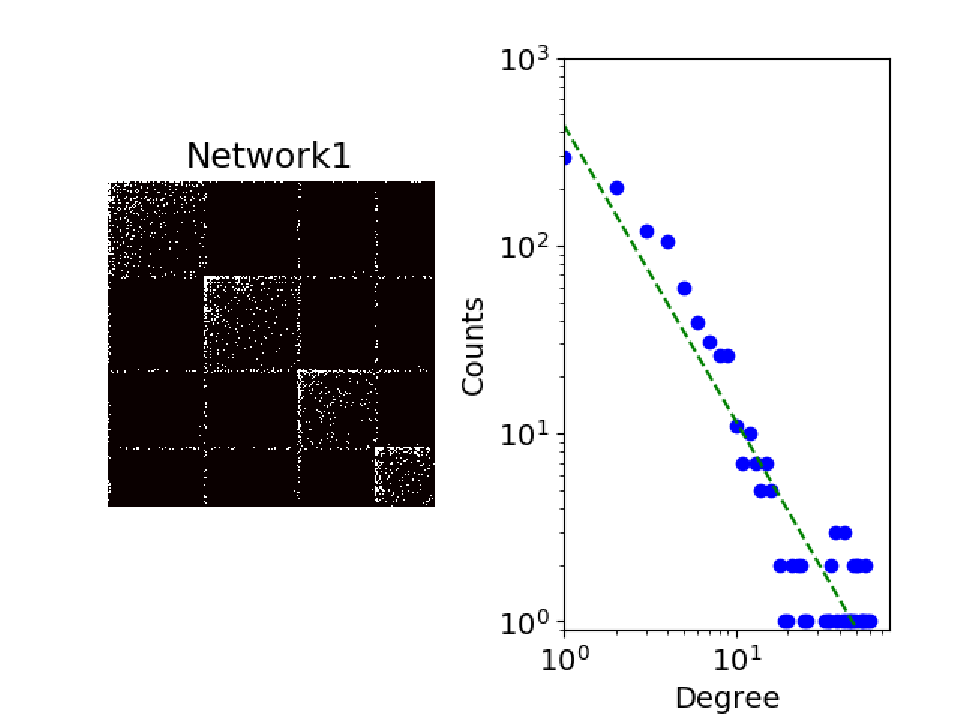
\includegraphics[width=\textwidth]{img/corpus/network1_dd}
        \end{minipage}
        \begin{minipage}{0.4\textwidth}
            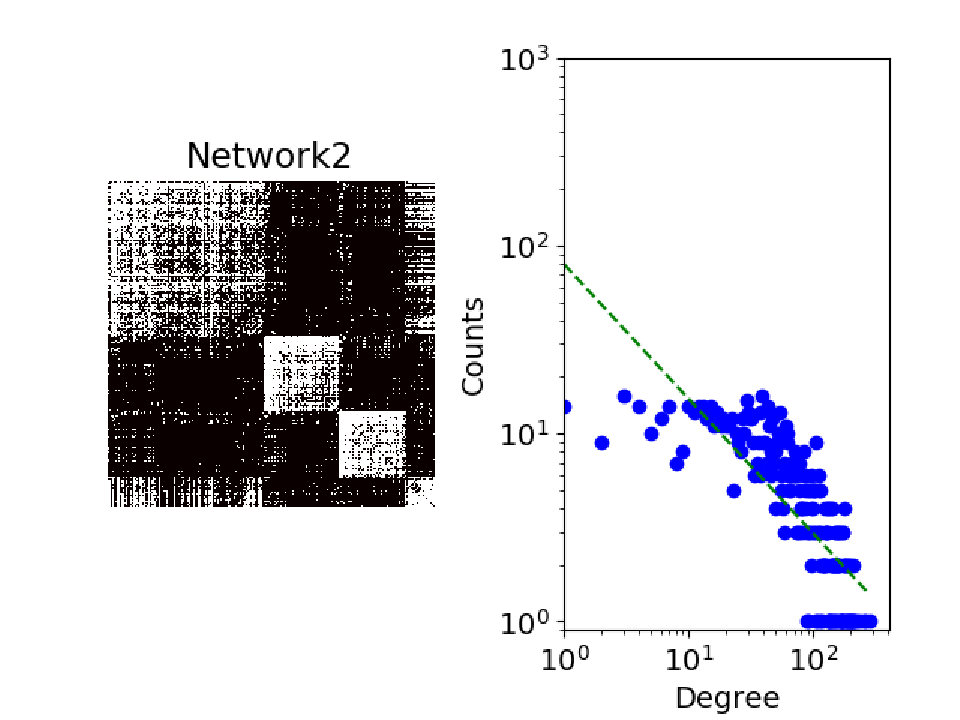
\includegraphics[width=\textwidth]{img/corpus/network2_dd}
        \end{minipage}
        %\vskip\baselineskip
        \begin{minipage}{0.4\textwidth}
            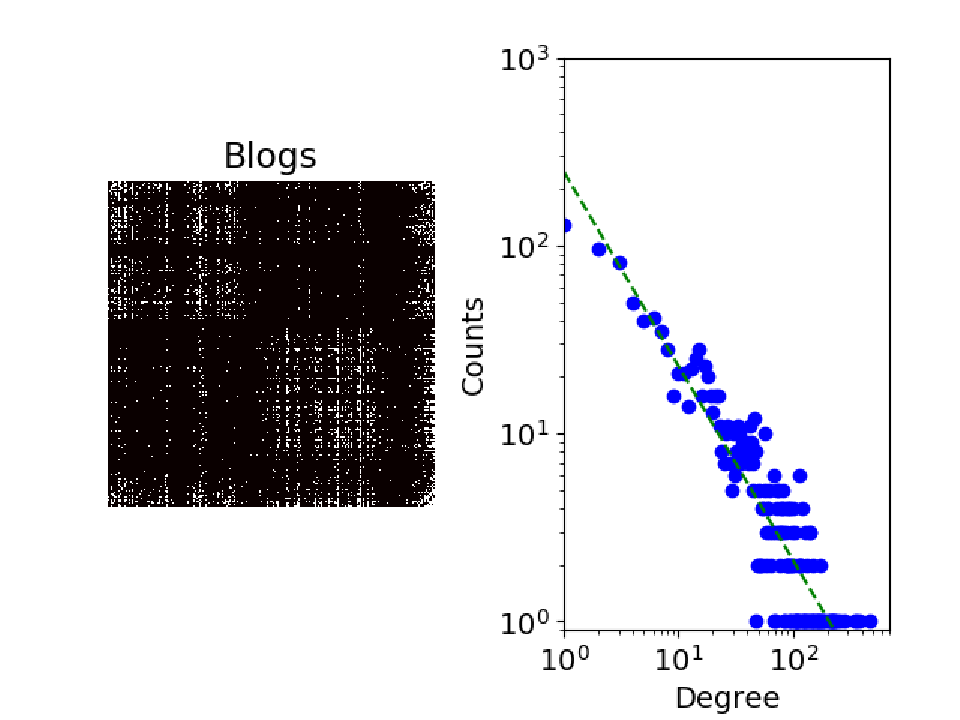
\includegraphics[width=\textwidth]{img/corpus/blogs_dd}
        \end{minipage}
        \begin{minipage}{0.4\textwidth}
            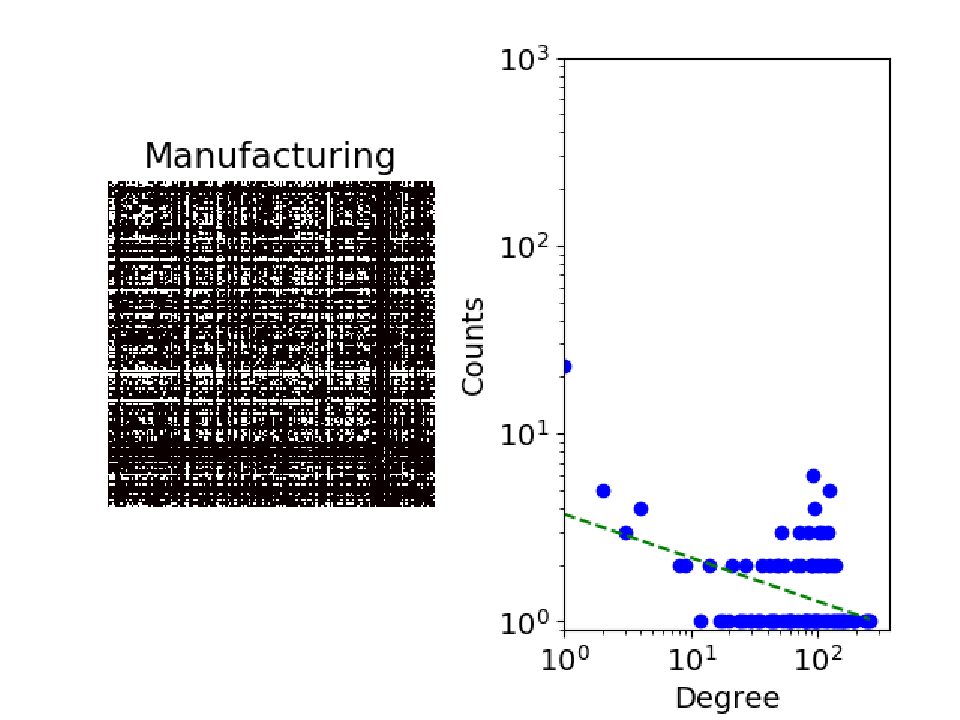
\includegraphics[width=\textwidth]{img/corpus/manufacturing_dd}
        \end{minipage}
	\caption{Adjacency matrices (left) and global degree distributions (right) for the four training datasets. In the adjacency matrices, a white dot corresponds to a 1 and a black dot to a 0.}
	\label{fig:corpuses}
\end{figure}

\begin{figure}[h]
    \centering
        \begin{minipage}{0.45\textwidth}
            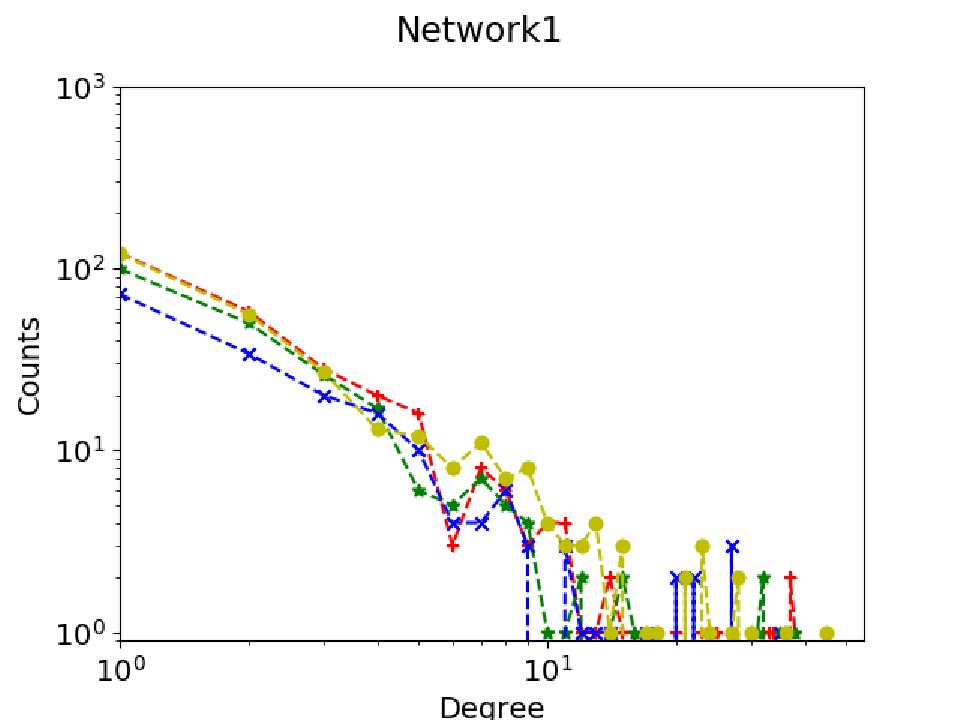
\includegraphics[width=\textwidth]{img/corpus/network1_1}
        \end{minipage}
        \begin{minipage}{0.45\textwidth}
            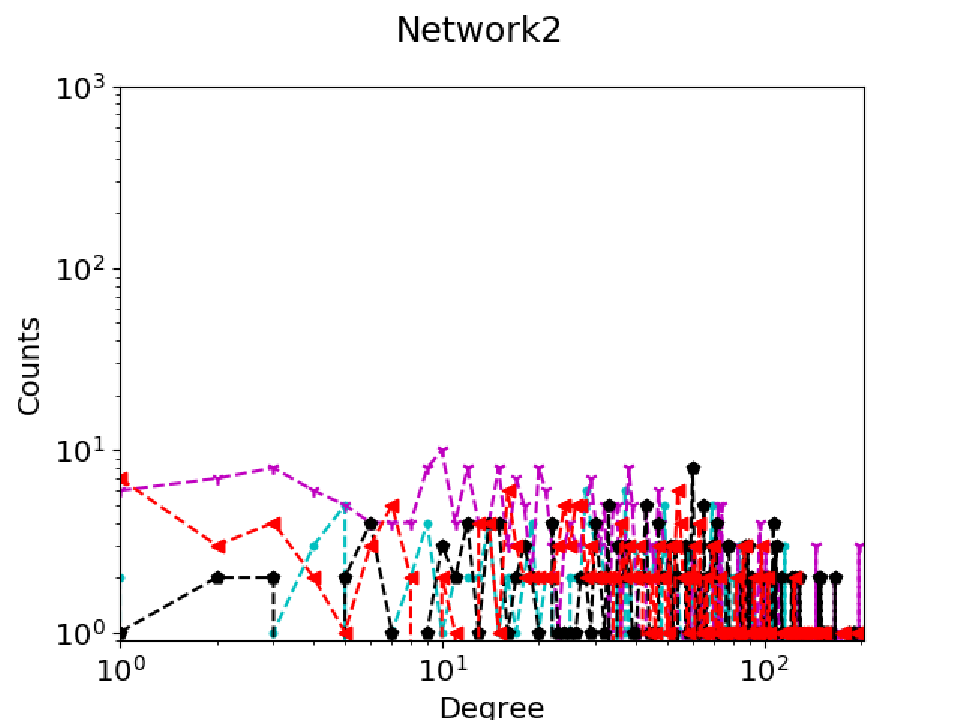
\includegraphics[width=\textwidth]{img/corpus/network2_1}
        \end{minipage}
        \vskip\baselineskip
        \begin{minipage}{0.45\textwidth}
            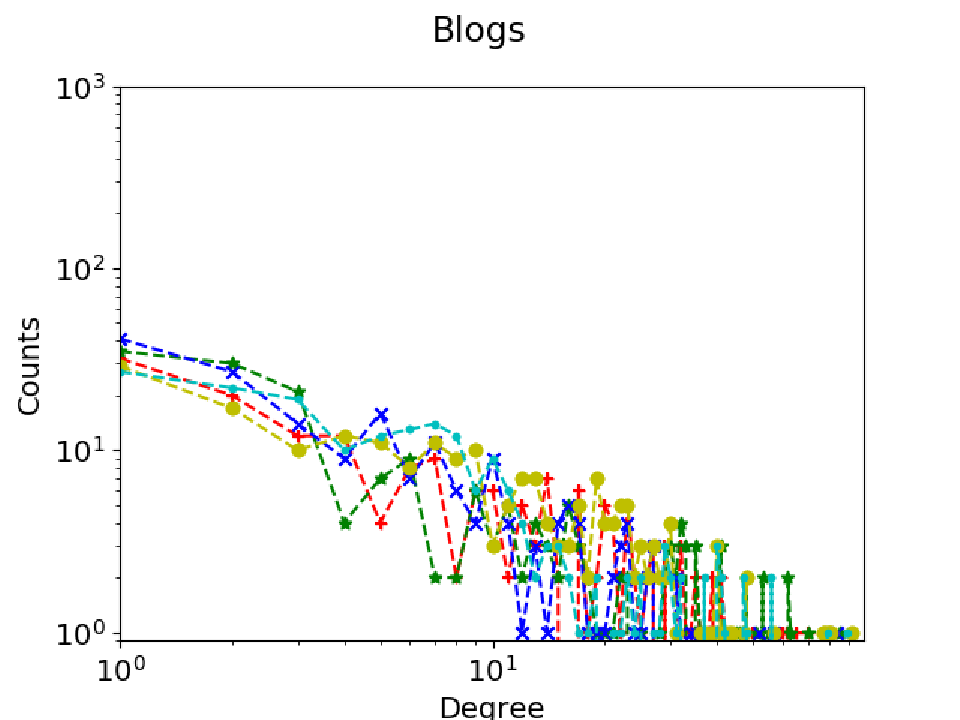
\includegraphics[width=\textwidth]{img/corpus/blogs_1}
        \end{minipage}
        \begin{minipage}{0.45\textwidth}
            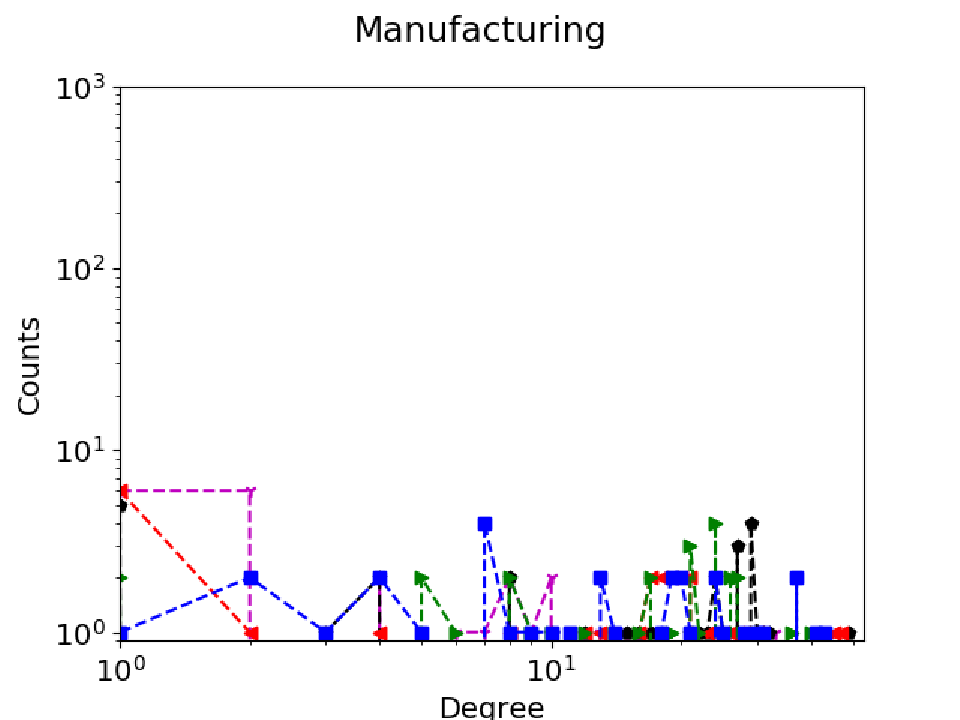
\includegraphics[width=\textwidth]{img/corpus/manufacturing_1}
        \end{minipage}
        \caption {Local degree distributions for the four training datasets. For Network1 and Network2 the classes come from ground-truth. For Blogs and Manufacturing, classes are obtained with a Louvain algorithm.}
	\label{fig:synt_graph_local}
\end{figure}



\subsection{Preferential attachment in $\M_e$}

For each dataset, we estimated the model parameters through a Markov Chain Monte Carlo inference consisting of 200 iterations. For \imb, the concentration parameters of HDP were optimized using vague gamma priors $\alpha_0 \sim \text{Gamma}(1,1)$ and $\gamma \sim \text{Gamma}(1,1)$ following \cite{teh2006hierarchical}. The parameters for the matrix weights  $\lambda_0$ and $\lambda_1$ were fixed to 0.1. For \ifm, the hyperparameter  $\sigma_w$ was fixed to 1 and the IBP hyperparameter $\alpha$ to 0.5. %in order to  have comparable number of classes with \imb.
Once the models have been learned, they are used to generate links (or non-links) between the entire set of network nodes. The whole procedure is repeated 10 times and the average values are reported as final results.


\begin{table}[h]{Preferential attachment measures for training datasets and networks generated with fitted models.}
\begin{tabular}{lrrrr}
  \multirow{2}{*}{\textbf{Training Datasets}}  &
  \multicolumn{2}{c}{Global} & \multicolumn{2}{c}{Local}\\
  \cmidrule(r){2-3} \cmidrule(l){4-5}
  &   $p$-value &   $\alpha$   & $p$-value & $\alpha$   \\
\hline
Network1       & 1 & 2.4 &   1.0 $\pm$ 0.0  &  1.8 $\pm$ 0.03  \\
Network2       & 0 & 1.3 &   0.0 $\pm$ 0.0  &  1.2 $\pm$ 0.01 \\
Blogs          & 1 & 1.5 &   1.0 $\pm$ 0.0  &  1.4 $\pm$ 0.03\\
Manufacturing  & 0 & 1.4 &   0.4 $\pm$ 0.3  &  1.3 $\pm$ 0.05 \\
\hline

  \ \textbf{\immsb} &&&& \\
\hline
Network1       & 0.9 & 1.4 &   1.0 \(\pm\) 0.0   &  3.5 \(\pm\) 0.7 \\
Network2       & 0 & 1.3 &   0.9 \(\pm\) 0.0   &  1.6 \(\pm\) 0.2 \\
Blogs          & 1 & 1.3 &   1.0 \(\pm\) 0.0   &  4.3 \(\pm\) 1.1 \\
Manufacturing  & 0 & 1.2 &   0.9 \(\pm\) 0.01  &  1.6 \(\pm\) 0.1 \\
\hline

  \ \textbf{\ilfm} &&&& \\
\hline
Network1      & 1 & 1.4 &   1.0 \(\pm\) 0.0  &  1.7 \(\pm\) 0.1 \\
Network2      & 0 & 1.2 &   0.0 \(\pm\) 0.0 &  1.2 \(\pm\) 0.0 \\
Blogs         & 1 & 1.3 &   0.9 \(\pm\) 0.2  &  1.5 \(\pm\) 0.1 \\
Manufacturing & 0 & 1.2 &   0.3 \(\pm\) 0.3  &  1.3 \(\pm\) 0.0 \\
\hline
\end{tabular}
\label{table:me_gofit}
\end{table}


\subsubsection{Degree distributions}

Table \ref{table:me_gofit} reports the value of the power-law goodness of fit for \imb\ and \ifm\ in the global case (left) and in the local case (right). The precision of the test was set to $\epsilon = 0.03$. It appears that for both models, the global preferential attachment is only verified for networks generated from datasets where the property was observed, namely in Network1 with p-value equal to 0.9 for \imb\ and 1 for \ifm, and in Blogs with a p-value equal to 1 for both models; the property is not verified in Network2 and in Manufacturing, where the p-values are equal to 0. This is in accordance with Proposition 2.1 according to which both \ifm\ and \imb\ do not satisfy global preferential attachment. However, these models are able to capture this property if it exists in the training datasets.  Moreover, one can observe that, in the local case, \imb\ complies with the preferential attachment with $p$-values equal or close to 1 for the four networks, while \ifm\ obtained low p-values for the networks that were less locally bursty (respectively  0  for Network2 and 0.3 for Manufacturing). In addition, the power-law coefficients $\alpha$ are significantly greater for \imb\ than for \ifm, and specially for the bursty networks Network1 and Blogs.

Figure \ref{fig:me_local} illustrates the local preferential attachment for Network1 (top) and Network2 (bottom) estimated with \imb\ (left) and \ifm\ (right). The shape of the local degree distributions appears more linear for \imb\ and with more fluctuations for \ifm. This illustrates the fact that \ifm\ does not capture local preferential attachment whereas \imb\ does, as stated in Proposition~\ref{prop:IMBlocal}.


\begin{figure}[h]
    \centering
    \begin{minipage}{0.4\textwidth}
        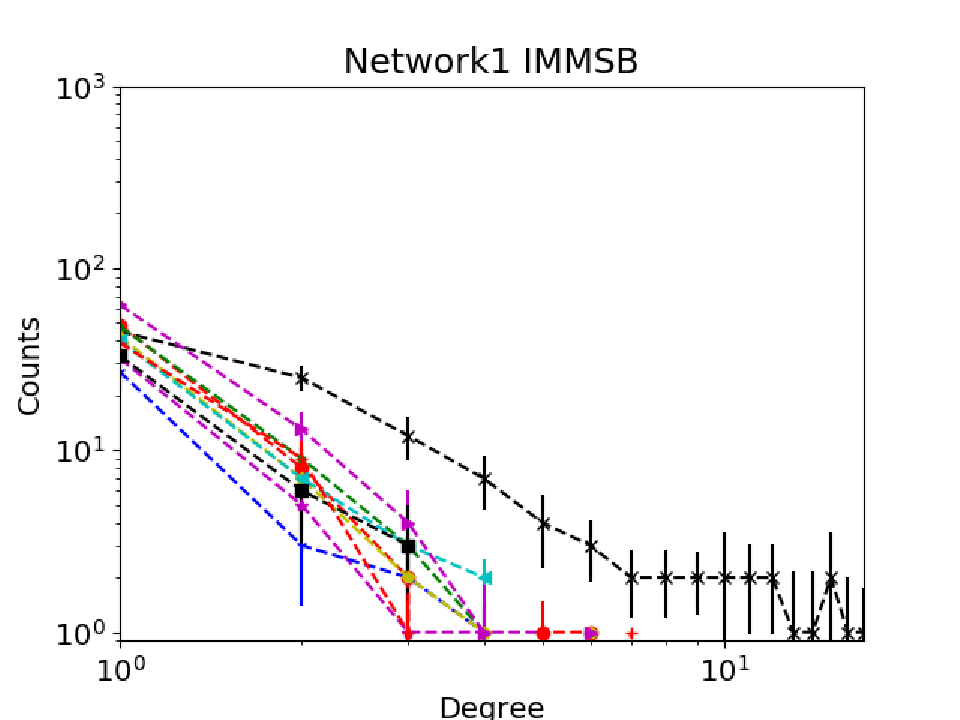
\includegraphics[width=\textwidth]{img/corpus/immsb_network1_1}
    \end{minipage}
    \begin{minipage}{0.4\textwidth}
        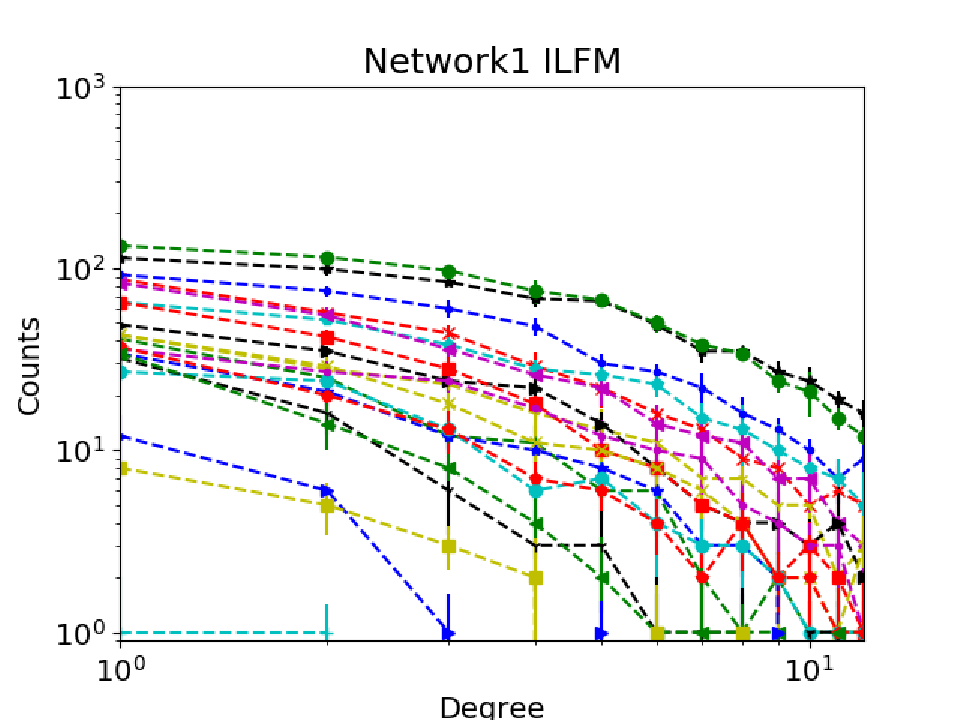
\includegraphics[width=\textwidth]{img/corpus/ilfm_network1_1}
    \end{minipage}
    \vskip\baselineskip
    \begin{minipage}{0.4\textwidth}
        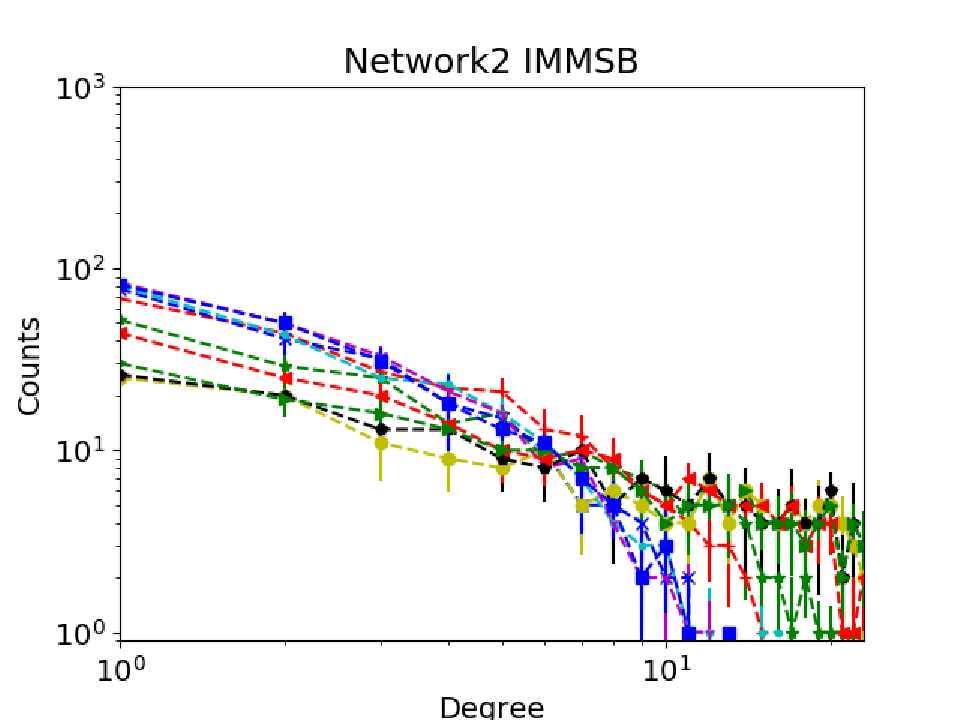
\includegraphics[width=\textwidth]{img/corpus/immsb_network2_1}
    \end{minipage}
    \begin{minipage}{0.4\textwidth}
        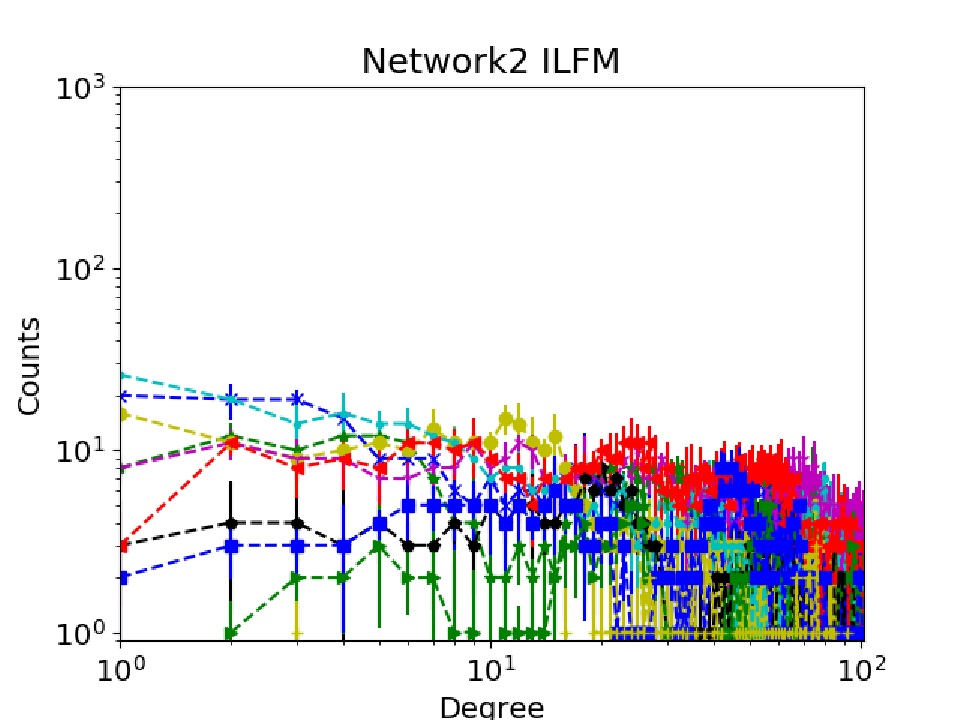
\includegraphics[width=\textwidth]{img/corpus/ilfm_network2_1}
    \end{minipage}
    \caption {Local degree distributions for Network1 (top row) and Network2 (bottom row) generated with fitted models \imb\ (first column) and \ifm\ (second column).} 
\label{fig:me_local}
\end{figure}



\subsubsection{Generating process}
In Figure \ref{fig:burst_immsb} and \ref{fig:burst_ilfm} we show respectively for IMMSB and ILFM the evolution of the local preferential attachment following the definition given in section \ref{sec:local_me}, for the networks Manufacturing and Networks1 and for two different values of the generating process step $p$ ($p$ is given as a percentage of $N$ in the plots). For IMMSB one can see on figure \ref{fig:burst_immsb}, that the probability of generating new links increases with the degree. However, for ILFM, one can observe, on figure \ref{fig:burst_ilfm}, some classes where the preferential attachment is no true such as for the class 3 in Manufacturing where the probability to generate new links decreases with the degree or contains some plateau. For Networks1, the probability to generate new links increases in average because the model is fitted with a networks where the preferential attachment is present. However, on can see that the increase of the probability is not as clear than for IMMSB. The value of the probability fluctuate and reaches some plateau. The interpretation of these results with regard to the properties that we asses for the local preferential attachment is that IMMSB is better adapted than ILFM to capture the local preferential attachment.


\begin{figure}[h]
\centering

% pmk PNAS3 -x prop2_process_local_me 85 95 -m immsb_cgs -c generator7 manufacturing

\begin{subfigure}
     \centering
         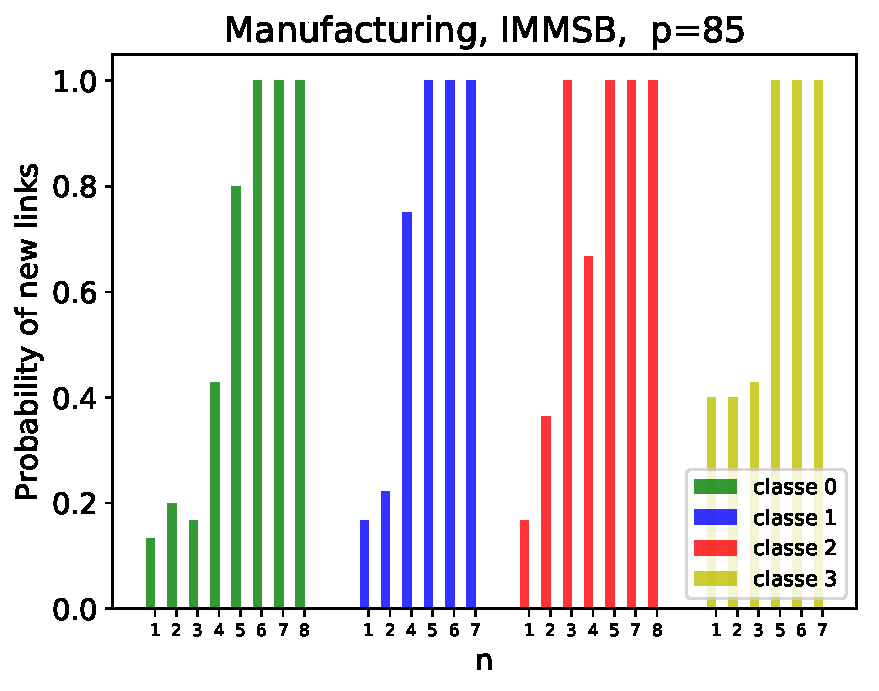
\includegraphics[width=0.45\textwidth]{img/burst/3_prop2_process_local_me__85}
\end{subfigure}
\begin{subfigure}
         \centering
      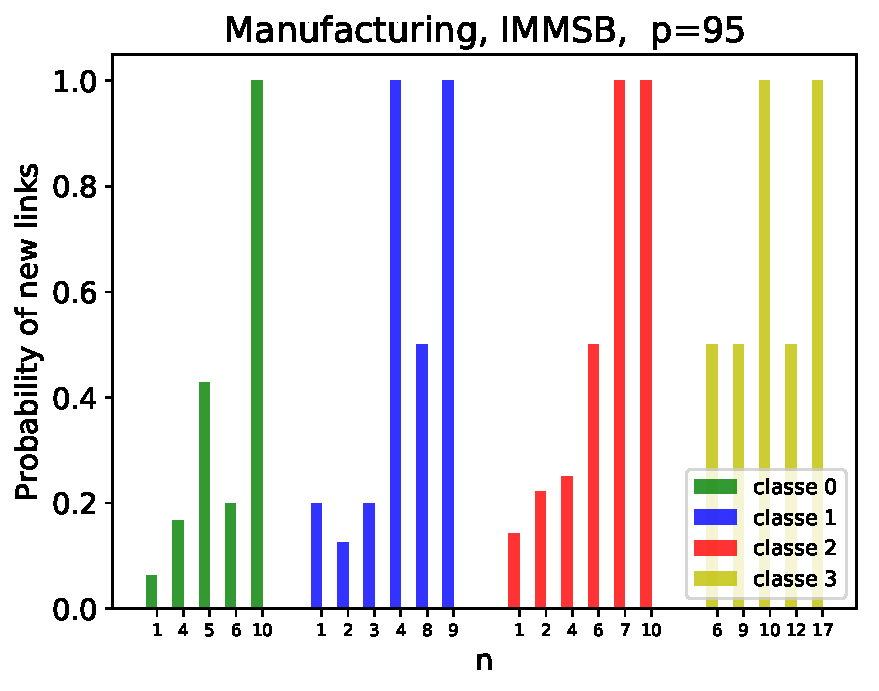
\includegraphics[width=0.45\textwidth]{img/burst/3_prop2_process_local_me__95} 
\end{subfigure}                                                                          
\begin{subfigure}                                                                        
         \centering                                                                      
      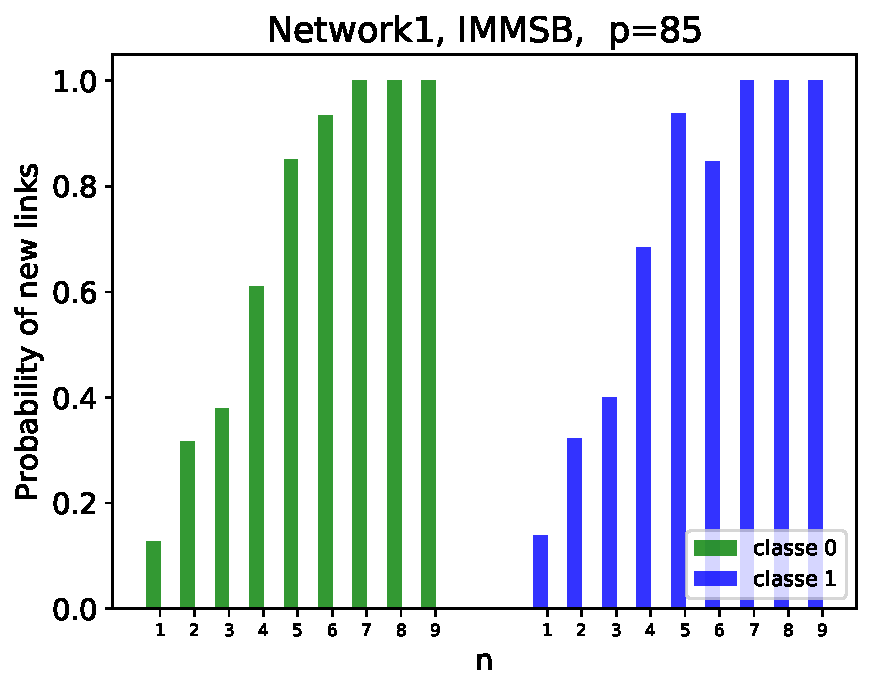
\includegraphics[width=0.45\textwidth]{img/burst/5_prop2_process_local_me__85}
\end{subfigure}                                                                          
\begin{subfigure}                                                                        
         \centering                                                                      
      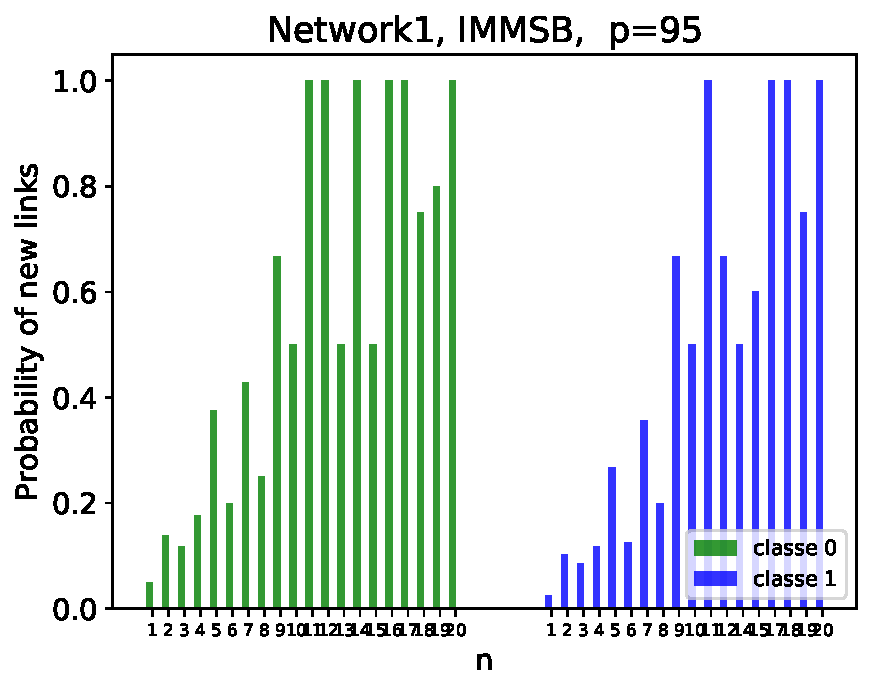
\includegraphics[width=0.45\textwidth]{img/burst/5_prop2_process_local_me__95}
\end{subfigure}                                                                          
\caption{Local burstiness process for IMMSB illustrated by the probability to generate new links for degree at step $p$. The model is fitted with the Manufacturing and networks1 networks for respectively line 1 and 2. First row is for a value of the generating step $p=85\%$(percentage of total number of nodes $N$ and $p=95\%$ for the second row . }
\label{fig:burst_immsb}



\end{figure}

\begin{figure}[h]
\centering

% pmk PNAS3 -x prop2_process_local_me 85 95 -m ilfm_cgs -c generator7 manufacturing 

\begin{subfigure}
     \centering
         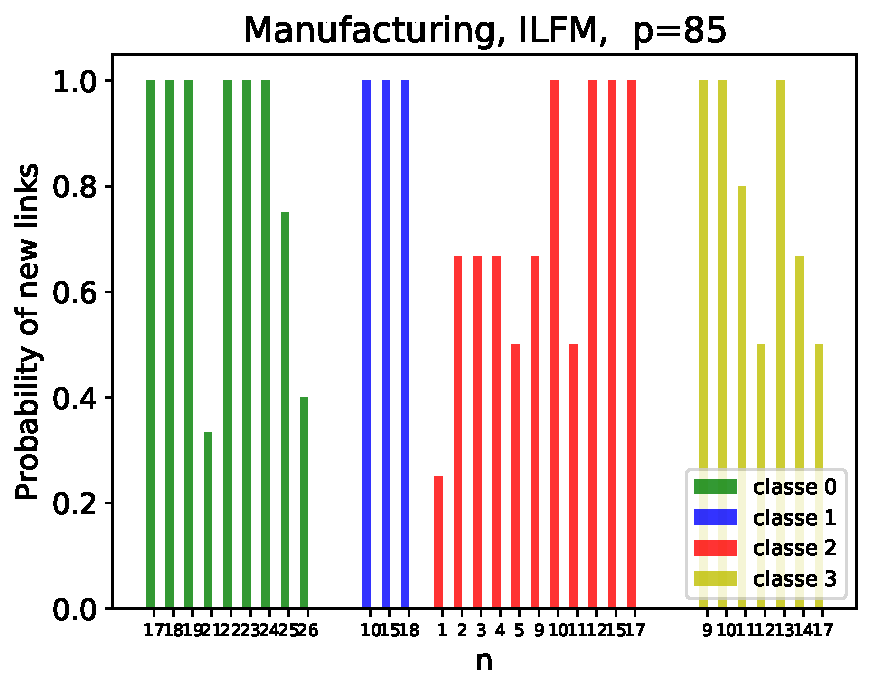
\includegraphics[width=0.45\textwidth]{img/burst/2_prop2_process_local_me__85}
\end{subfigure}
\begin{subfigure}
         \centering
      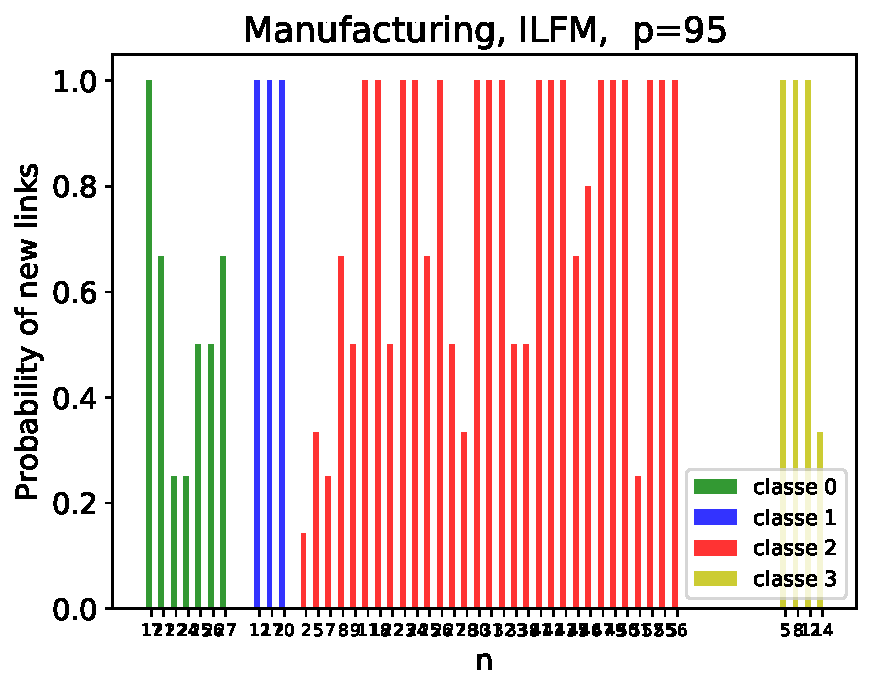
\includegraphics[width=0.45\textwidth]{img/burst/2_prop2_process_local_me__95} 
\end{subfigure}                                                                          
\begin{subfigure}                                                                        
         \centering                                                                      
      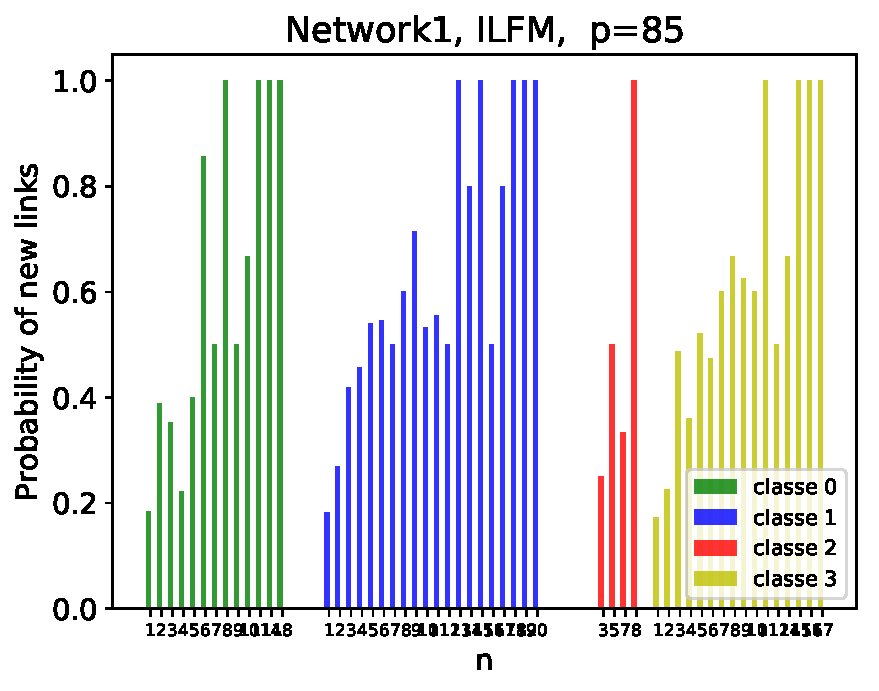
\includegraphics[width=0.45\textwidth]{img/burst/4_prop2_process_local_me__85}
\end{subfigure}                                                                          
\begin{subfigure}                                                                        
         \centering                                                                      
      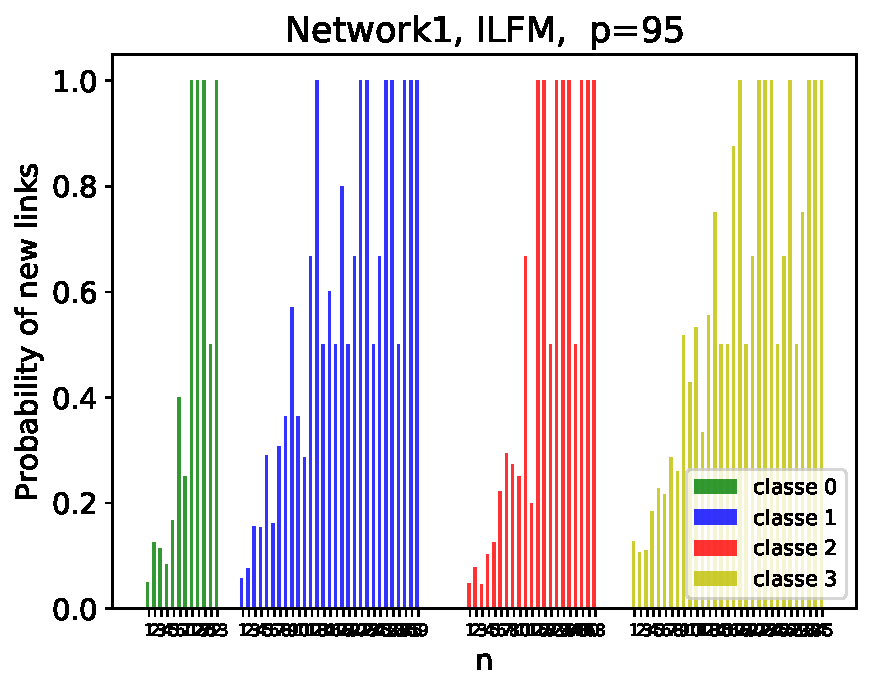
\includegraphics[width=0.45\textwidth]{img/burst/4_prop2_process_local_me__95}
\end{subfigure}                                                                          
\caption{Local burstiness process for ILFM illustrated by the probability to generate new links for degree at step $p$. The model is fitted with the Manufacturing and networks1 networks for respectively line 1 and 2. First row is for a value of the generating step $p=85\%$(percentage of the total number of nodes $N$ and $p=95\%$ for the second row . }
\label{fig:burst_ilfm}



\end{figure}

\subsubsection{Performance evalutation}

%% efficacy != efficiency

in Figure \ref{fig:auc}, we compare the performance of the models for predicting new links using the Area Under the Curve (AUC) measure as a function of the training set size. In the bottom plot, the y-axis gives the relative performance defined as the difference of the AUC values for \imb\ and \ifm\ ($AUC_{\imb} - AUC_{\ifm}$) whereas the x-axis indicates the percentage of links randomly removed from the datasets and used as test examples. Hence, the number of training data decreases with the x-axis and a positive value on the y-axis indicates that \imb\ outperforms \ifm.  The relative performance corresponds to the difference of the best AUC values obtained for both models on the 10 inference experiences. The top plots illustrate a case where 75 percent of the data is used as test set and where \imb\ dominates \ifm\ on Network1 (left), and the opposite on Network2 (right).

In general, as shown in the bottom plot, \ifm\ obtains better performance than \imb. However, the relative predictive performance of \imb\  increases  when the quantity of training data decreases on bursty networks, whereas for non-bursty networks the results are the opposite: the performance of \ifm\ increases when the size of the learning dataset decreases. This is particularly visible for Network2. The results for Manufacturing are less marked, which is certainly due to the small size of this network, making the prediction less challenging.

The above behavior can be explained by the fact that \imb\ satisfies the local preferential attachment whereas \ifm\ does not: as links are randomly removed, one is more likely to remove links from large classes than from small ones; a model that enforces local preferential attachment on bursty networks is thus more likely to reconstruct those removed links. This is what is happening on Network1 and Blogs for \imb. On the contrary, for non-bursty networks, a model enforcing local preferential attachment is penalized.

\begin{figure}[ht]
\centering
    \begin{minipage}{0.45\textwidth}
        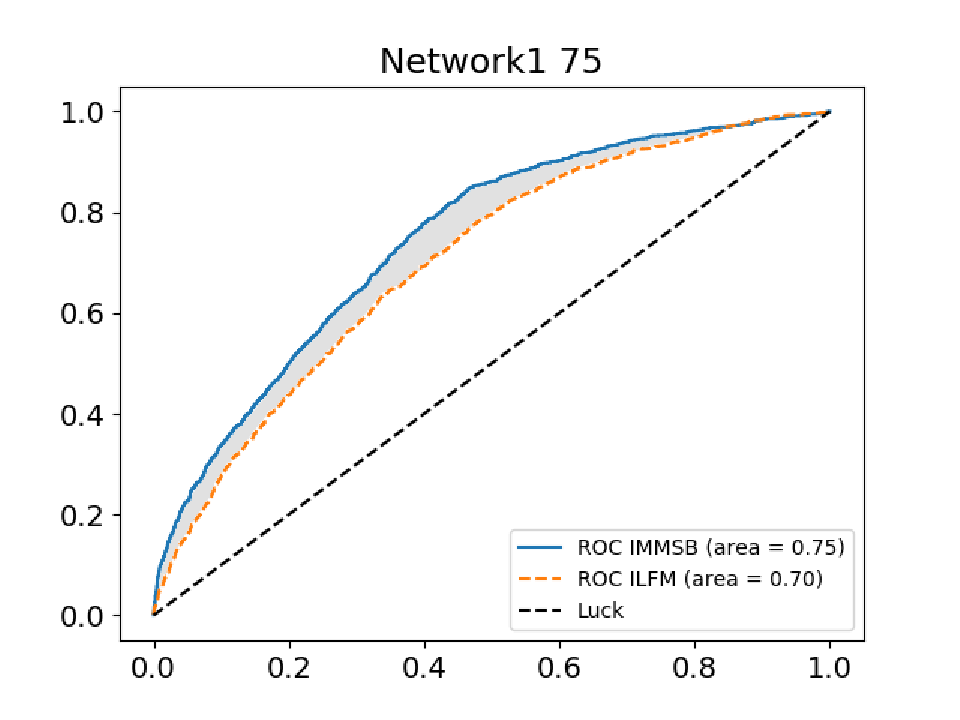
\includegraphics[width=\textwidth]{img/corpus/roc_network1_75_f}
    \end{minipage}
    \begin{minipage}{0.45\textwidth}
        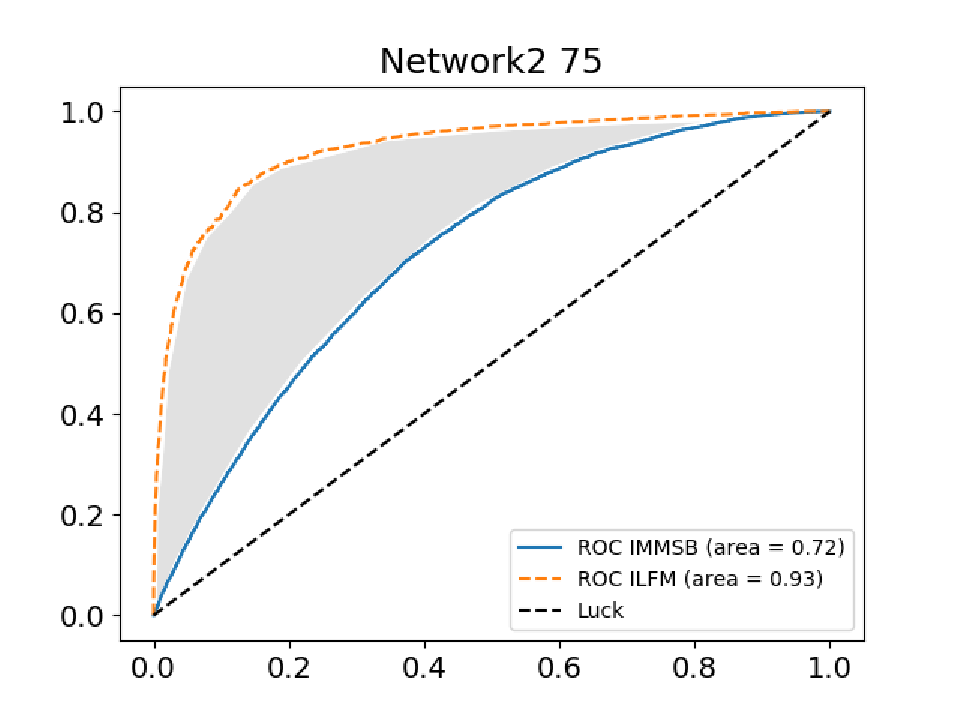
\includegraphics[width=\textwidth]{img/corpus/roc_network2_75_f}
    \end{minipage}
    \begin{minipage}{0.5\textwidth}
        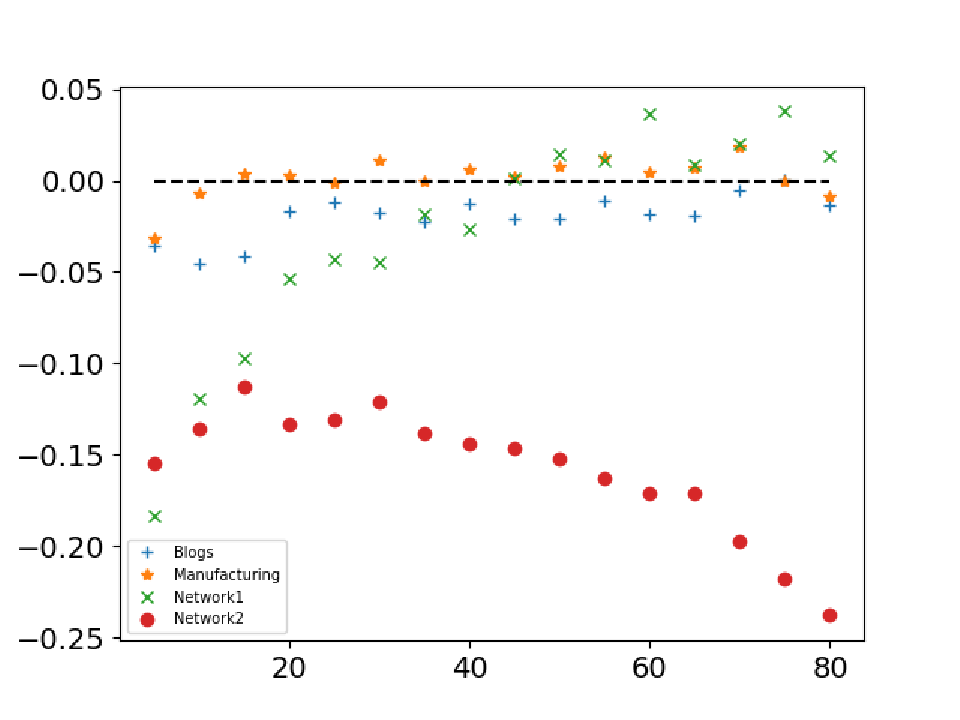
\includegraphics[width=\textwidth]{img/corpus/testset_max_20}
    \end{minipage}
    \caption{Top: AUC-ROC curves for Network1 (left) and Network2 (right) with 75 percent of data used for learning that compares the performance of models. Bottom: Relative performance of \imb\ and \ifm\ according to the percentage of data used for testing, the rest being used for learning.}
\label{fig:auc}
\end{figure}


\subsection{Preferential attachment in $\M_g$}

Illustrations in the $\M_g$ case are based on the simulation of the models where the parameters $F$ and $\Phi$ have been marginalized out. In other words the degrees that we are going to observe are the expected degree for a large numbers (in the sense of the theory of large numbers) of generated parameters, given the hyper-parameters of the model. In order to simulate this scenario, we generated a large number (100) of networks with a given set of hyper-parameters for the models. Then we reported the average global degree distribution in Figure \ref{fig:mg_deg} (top).  For  this  experiments, fix the number of nodes to 1000. We went trough the generative process 100 times in order to simulate the $\M_g$ mode. In order to have a comparable number of classes for \ifm\ and \imb\ and block-block probability priors, we fix the hyper-parameters  $\lambda_0=\lambda_1=0.5$ for both models,  $\alpha=\alpha_0=1$ for \ifm, and  $\gamma=0.5$ for \imb.

We see that the global degree distributions are not monotone, with several peaks, and that the range values of the outcome degrees are concentrated in a small segment determined by the hyper-parameters of the models. The shape of the global degree distributions shows that the global preferential attachment is not satisfied.


In the Figure \ref{fig:mg_deg} (bottom), we also reported a measure on the local preferential attachment in $\M_g$. An important note is that, to be able to compute the statistics for the local degree, the latent classes need to be aligned between the different epochs in order to report average values of the local degree distributions. But, the mixed membership models do not defined unique labels over the latent classes. Thus, it is not straightforward to identify the common classes between the generations of the different network realizations. Actually, as the processes are exchangeable, they is no strict correspondence between classes in two independent generative process. Nevertheless, the property of the Dirichlet Process and the Indian Buffet Process, enable to identify the classes by ordering them with their size (or concentration). For example, the stick breaking process interpretation of the DP provides a natural class ordering with a descending (or ascending) order of the class representations. While the IBP generates a row-exchangeable feature matrix, it is possible to reorder the rows to obtain a $F$ matrix where the size of the classes keeps the same descending (or ascending) order.

For the local degree, one can see that, for IMMSB, the shape of the distributions is characteristic of the preferential attachment effect (linear decrease in a log-log space) while it is not the case for ILFM. This experiment is interesting as it show that, for \imb, the local preferential attachment property in $\M_e$ seems to holds also in $\M_g$.

% Degree distribution in MG
%  2x2 figure  
%  [global immsb] [global ilfm]
%  [local ilfm] [gloal ilfm]
%
% pmk PNAS3 -x gennetwork burstiness -g -c generator7 -n 1000 --epoch 100


\begin{figure}[h]
    \centering
    \begin{minipage}{0.45\textwidth}
        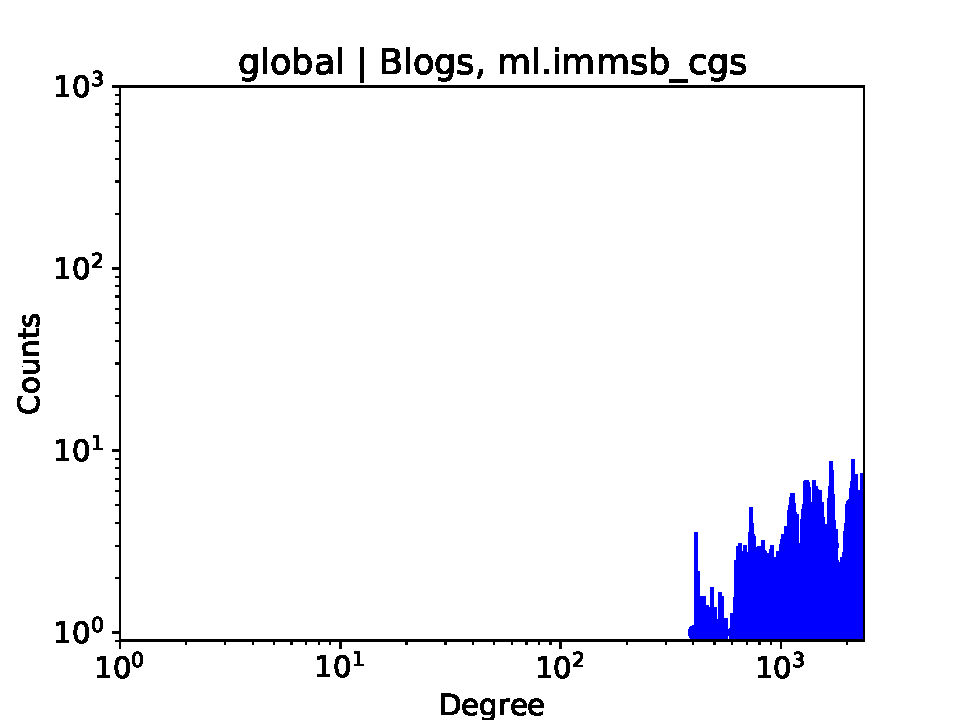
\includegraphics[width=\textwidth]{{{img/0201/MG_ml.immsb_cgs_0}}}
    \end{minipage}
    \begin{minipage}{0.45\textwidth}
        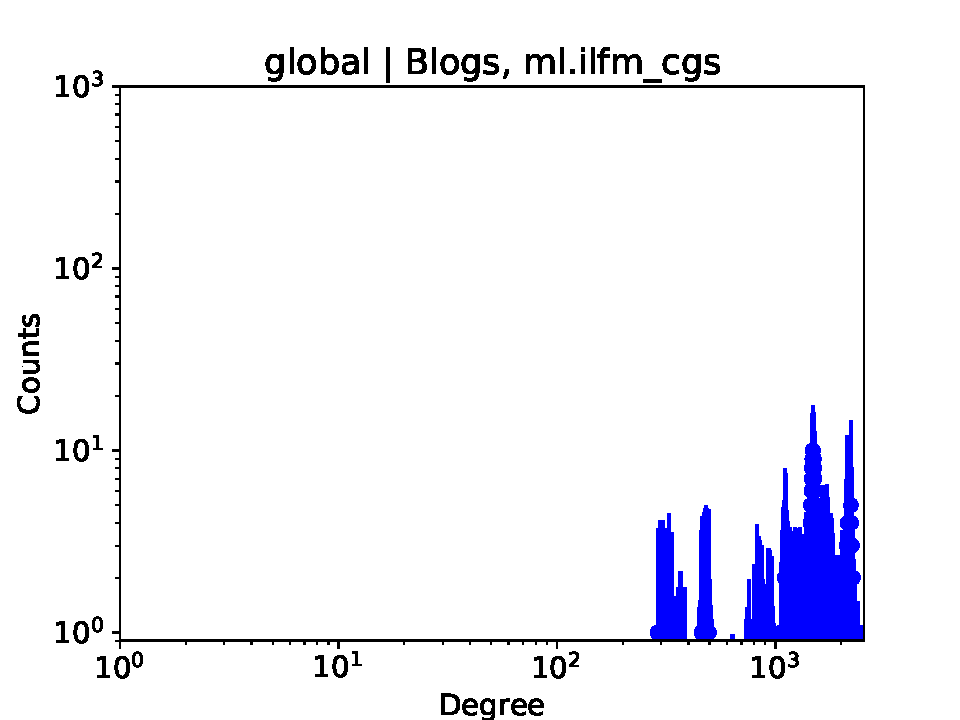
\includegraphics[width=\textwidth]{{{img/0201/MG_ml.ilfm_cgs_0}}}
    \end{minipage}
    \vskip\baselineskip
    \begin{minipage}{0.45\textwidth}
        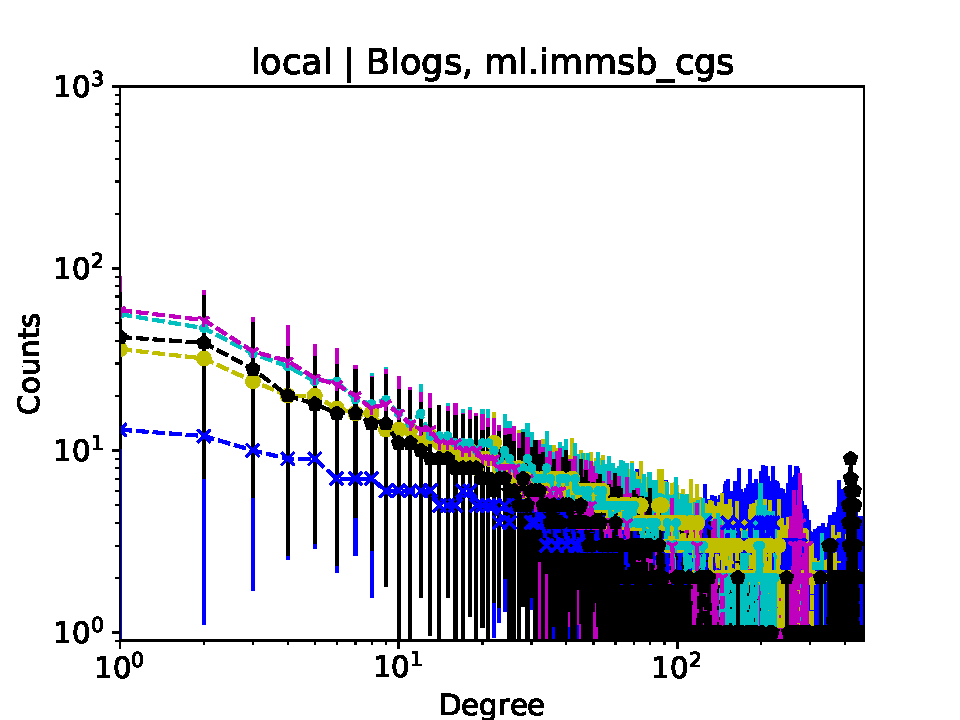
\includegraphics[width=\textwidth]{{{img/0201/MG_ml.immsb_cgs_1}}}
    \end{minipage}
    \begin{minipage}{0.45\textwidth}
        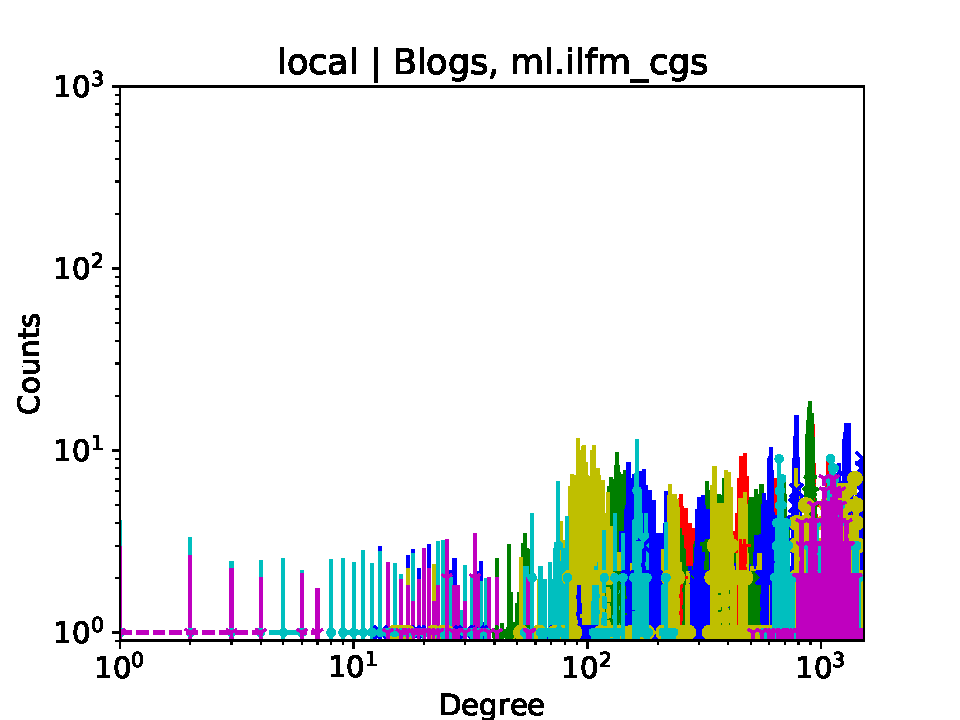
\includegraphics[width=\textwidth]{{{img/0201/MG_ml.ilfm_cgs_1}}}
    \end{minipage}
    \caption {Global degree distribution (top) and local degree distribution (bottom) from IMMSB (left) and ILFM (right) in the generative mode $\M_g$.} 
\label{fig:mg_deg}
\end{figure}



%Figures \ref{fig:mg_process} gives a simulation of the evolution of the expected (global and local) degree during the sampling process according to the equation \eqref{eq:degree_def}. We will refer this process as the degree count process which basically is a cummulative count over the nodes of the link measure (eitheir the true link/non-link observation for ILFM or the likelihood of a link for IMMSB) . Because, we observe the degree count averaged on all the nodes, we also plot the variance over the nodes of those degree count process.
%Interestingly, one can show that for both models, the global and local expected degree count processes follow a linear increase, while the variance of the degree count processes are slightly convex. Furthermore, it is more pronounced for IMMSB for the global degree while it seems that concerning the local degree, the models are not differentiable. Nevertheless, if we look at the standard deviation of the variance for each local degree we see that for IMMSB it seems to be correlated to the variance (the more variance (over nodes) in a local degree count, the more this variance can deviate. In other words, the variance over the epoch increase too.). This is an interesting interpretation of the source of emergence of the local preferential attachment for IMMSB.

%% Degree process (cumulative count) in MG
%  2x2 figure  
%  [glogal expectaion] [global variance]
%  [local expectation] [local variance]
%
% pmk PNAS3 -x burst_process_mg -g -c BA -n 200 --epoch 10
% pmk PNAS3 -x burst_process_local_mg -g -c BA -n 200 --epoch 100


\begin{figure}[h]
    \centering
    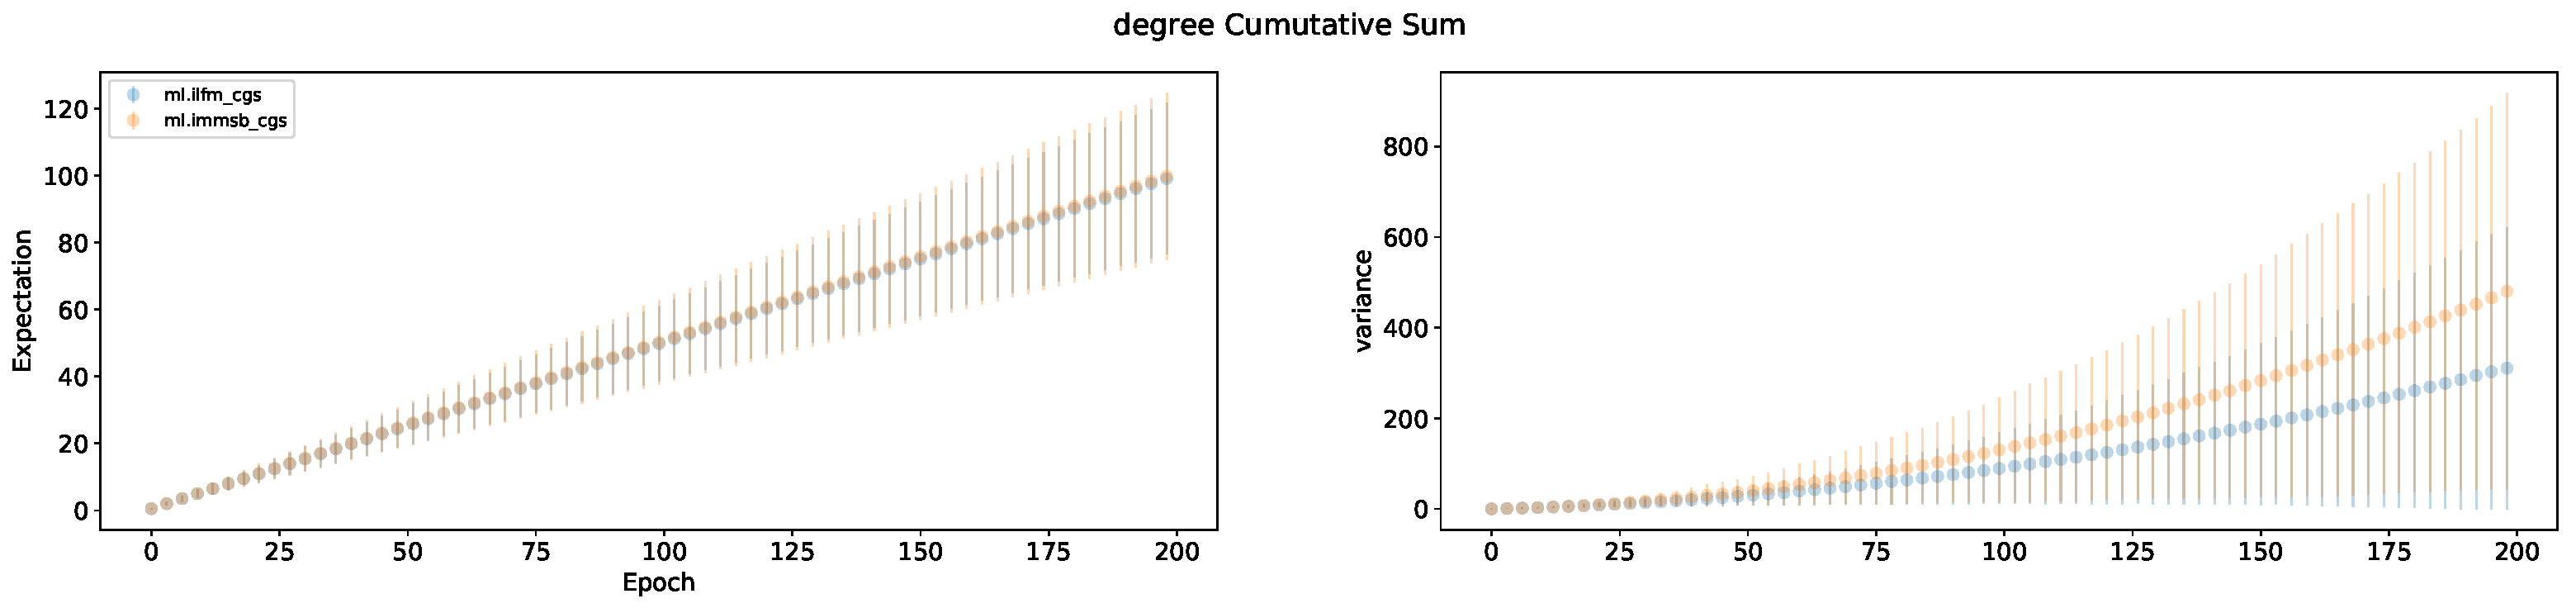
\includegraphics[width=\textwidth, height=6cm]{{{img/0201/BA_burst_process_mg_BA}}}
    \caption {The Left plot is the expectation of the degree count process over the nodes of the network. The right plot is the variance of the degree count process over the nodes of the network. The standard deviation of the curves is the deviation according to each epoch generation.} 
\end{figure}

\begin{figure}[h]
    \centering
    \begin{minipage}{0.99\textwidth}
        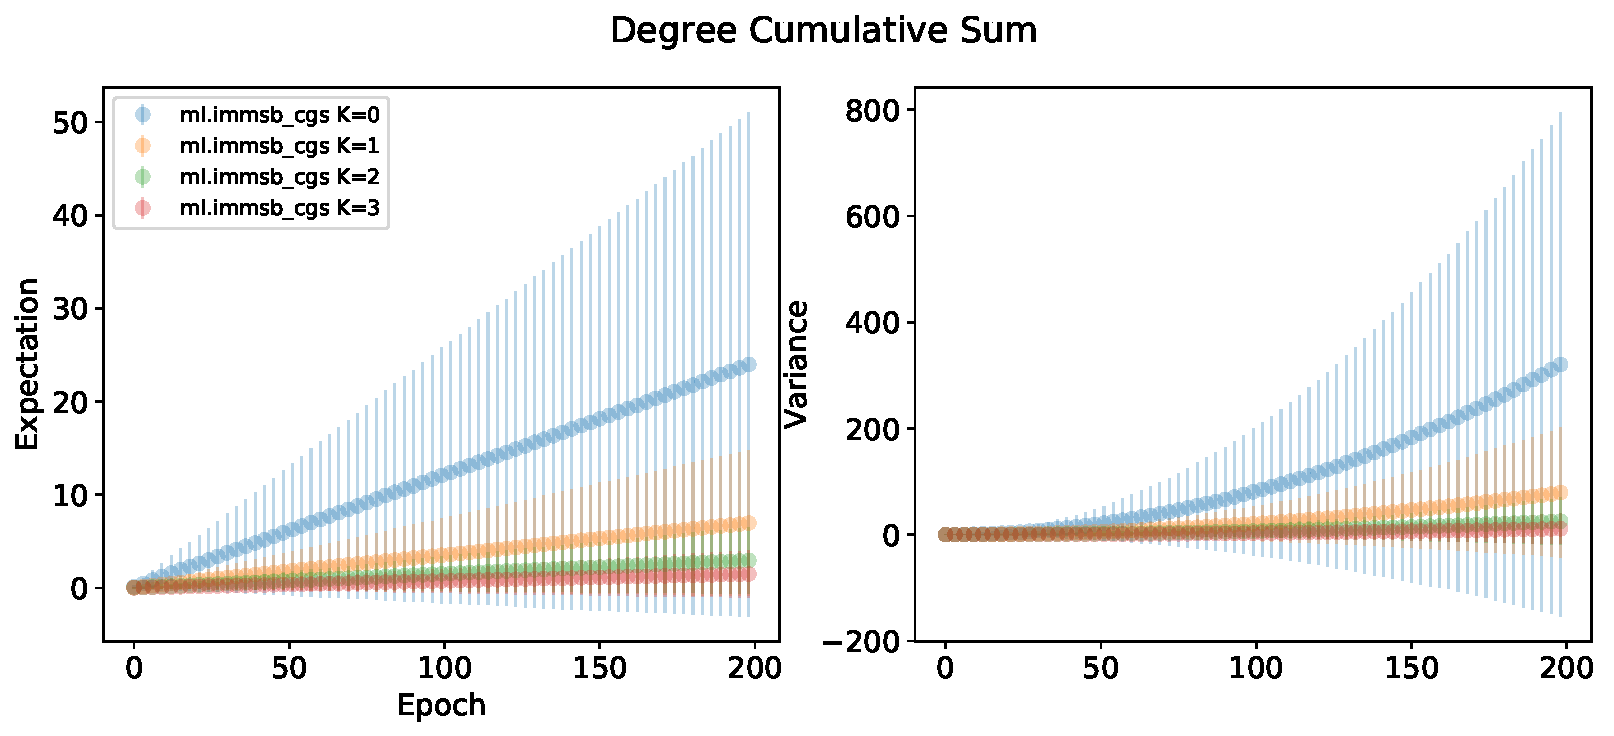
\includegraphics[width=\textwidth]{{{img/0201/ml.immsb_cgs_burst_process_local_mg_ml.immsb_cgs}}}
    \end{minipage}

    \begin{minipage}{0.99\textwidth}
        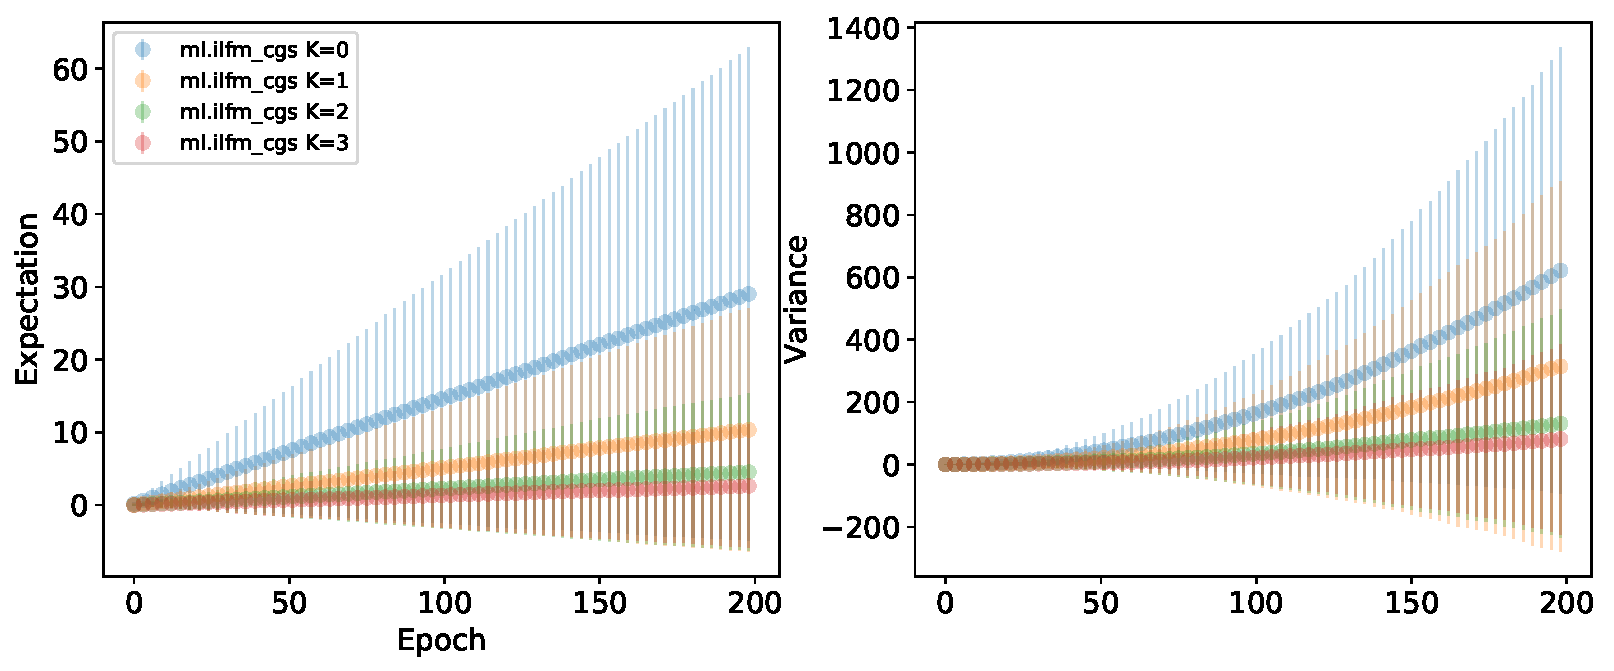
\includegraphics[width=\textwidth]{{{img/0201/ml.ilfm_cgs_burst_process_local_mg_ml.ilfm_cgs}}}
    \end{minipage}
    \caption {Top figure represent IMMSB local degree count process. The left part of the figure is the average overs the network's node and the roght part is the variance. Bottom figure is the same quantities but for ILFM model.} 
\label{fig:mg_deg}
\end{figure}






\section{Conclusion}
\label{sec:concl}

We have studied whether stochastic mixed membership models, such as \ifm\ and \imb\, can generate new links while satisfying properties frequently verified in real  social networks, namely homophily and preferential attachment. To do so, we have introduced formal definitions of these properties and have analyzed how these models behave according to those definitions. We have shown, in particular, that both models are \textit{homophilic} with the natural similarity that underlies them. Concerning preferential attachment, we have shown that stochastic mixed membership models do not comply with global preferential attachment. The situation is however more contrasted when the property is considered at the local level: \imb\ enforces local preferential attachment whereas \ifm\ does not.~\\

These findings have been validated experimentally on two real and two artificial networks that have different degrees of global and local preferential attachment. An important, practical finding of our study is that \imb, usually considered of lesser "quality" than \ifm, can indeed yield better results on bursty networks (\textit{i.e.} networks with preferential attachment) when the number of training data is limited.~\\

There are many directions to extend this work with the motivation of improving our theoretical understanding of graphical models for link prediction in complex networks. A straightforward extension is to examine the relation between the local preferential attachment and the dynamic of the latent classes.  
%For example, some special value of the hyperparameters, of the non-parametric priors, could lead to a very large number of classes or, at the opposite, just one class. Between these two extremes, that goes from a vanishing local aspect of the degree distribution to a number of classes that overfit the data, on can ask how this parameter affect the global and the local degree distribution of a random graph.  
For instance, a fundamental result is the Aldous-Hoover theorem, which implies that exchangeable random graphs cannot be sparse \cite{orbanz2015bayesian}. It seems that the sparsity is related in some way to the preferential attachment in a network. Thus, the following question arises: would it be realistic to assume the exchangeability hypothesis for the local case but not for the global case, and how this fact impacts the burstiness of the global degree distribution and the sparsity of the graph.

We believe that answering to those questions open a way to develop and design Bayesian models able to better capture the fundamental properties of  real social networks.


~\\ % don't compile if commented ?!
\bibliographystyle{chicago}
\bibliography{./a}

%\appendix
%\section{Appendix}
\label{sec:append}

\subsection{Mixed membership Models}
\label{sec:mixmembership}
In the Mixed Membership Models \cite{MMM}, the models can be defined at the link level by the likelihood of generating a link between two nodes given the contribution of each classes (or features). For IMMSB, this likelihood is straightforward, but for ILFM the class membership is defined deterministically by the binary vector $\mat{f}$. If the $k^{th}$ row is active (equal to one) then the node has the membership, else it doesn't. Hence for ILFM, We can write the likelihood  using the Dirac distribution $\delta(x)$ that gives one for $x=0$ as follows:

\begin{align}
    \pr(y_{ij} \mid \mat{F}, \mat{\Phi } ) &= \sigma \sum_{k, k'} \pr(y_{ij}\mid\phi_{k,k'}) \pr(k \mid \mat{f}_i) \pr(k' \mid \mat{f}_j) \\
    &=  \sigma \sum_{k, k'} \phi_{k,k'}  \delta(1-f_{ik}) \delta(1-f_{jk'})
    \end{align}
    

\subsection{Collapsed Gibbs sampling updates for IMMSB}

We provide here the derivation of the updates of the IMMSB model, described in Section~\ref{sec:models}.

%From the definition of the model, one has: $\pr(z_{ij} = k \mid \mat{f}_i) = f_{ik}$.

%\textcolor{red}{Adrien, peux-tu donner la d\'erivation ? La forme actuelle n'est valable que pour MMSB.} 

%heeeere \alpha is \alpha_0

Inference for the IMMSB model by using the Collapse Gibbs sampler gives updates for class assignment $Z \in N\times N \times 2$ for each interactions $Y \in N\times N$. Thus for all pair of interaction (i,j) we jointly sample the classes $(z_{ij}, z_{ji})$ who implicitly, take the values $(k,k')$ :
\begin{align} \label{eq:cgs}
&\pr(z_{ij}, z_{ji} \mid Z^-, Y,  \mat{\beta}, \alpha, \mat{\lambda} )  \\
&\propto\pr(z_{ij}, z_{ji} \mid Z^-, \alpha,\mat{\beta}) \pr(y_{ij} \mid Y^{-ij},  Z^-,z_{ij}, z_{ji},  \mat{\lambda} ) \nonumber
\end{align}
The term $Z^-$ denote that both $z_{ij}$ and $z_{ji}$ are exclude from $Z$. We now treat the first term of equation \ref{eq:cgs}.  
\begin{align}
& \pr(z_{ij}, z_{ji} \mid Z^-, \alpha,\mat{\beta})\\
&\propto \pr(z_{ij} \mid \mat{z}_i^{-j}, \mat{z}_j, \alpha,\mat{\beta})  \pr(z_{ji} \mid \mat{z}_j^{-i}, \mat{z}_i, \alpha,\mat{\beta}) \nonumber
\end{align}
Let's consider the density of $z_{ij}$:
\begin{align}
&\pr(z_{ij} \mid \mat{z}_i^{-j}, \mat{z}_j, \alpha,\mat{\beta}) \propto \pr(z_{ij},  \mat{z}_i^{-j}, \mat{z}_j, \alpha,\mat{\beta}) \\
&= \int_{f_i} \pr(f_i \mid \mat{\beta}, \alpha) \pr(z_{ij} \mid f_i) \prod_{j_0\neq j} \pr(z_{ij_0} \mid f_i) \prod_{j_0 =  1}^N  \pr(z_{j_0 i} \mid f_i)  df_i \nonumber
\end{align}


Due to the an augmented representation of the Chinese Restaurant Franchise (CRF) with the Stick Breaking Process \cite{HDP}, the density of the features can be approximated by the following Dirichlet distribution;
\begin{equation}
f_i \mid \mat{\beta}, \alpha \sim Dir(\alpha \beta_1,..,\alpha\beta_K, \alpha\beta_{new})
\end{equation}
Where $\alpha\beta_{new}$ represent the contribution for sampling a new class. Since $\pr(z_{ij} \mid f_i)$ is drawn from a multinomial, the model is said to be conjugate and reduce to a simple closed form expression:
\begin{enumerate}
\item If the class $k$ has already been observed:
   \begin{align}
    \pr(z_{ij} =k \mid .) &\propto N_{ik}^{-ij} + \alpha_0 \beta_k
    \label{eq:update-immsb}
   \end{align}
\item In case of a new class $k_{new}$:
   \begin{align}
    \pr(z_{ij} =k_{new} \mid.) &\propto \alpha_0 \beta_{new} \nonumber   
   \end{align}
\end{enumerate}
 Where  $N_{ik}$ is the count for node $i$ being assigned to class $k$. As we show that the equations are symmetric, sampling for $z_{ji}$ is straightforward.

~\\
Again, referring the CRF, the sampling of the tables configuration $\mat{m}$ is given by: 
\begin{equation}
\pr(m_{ik} \mid Z, \bm{m}^{-ik}, \mat{\beta} ) = \frac{\Gamma(\alpha_0 \beta_k)}{\Gamma(\alpha_0 \beta_k + n_{j\bm{.   }k})} s(n_{j\bm{.}k}, m) (\alpha_0 \beta_k)^m
\end{equation}
And, finnaly  $\mat{\beta}$ is obtained by:
\begin{equation}
\mat{\beta} \sim Dir(m_1,.., m_K, \gamma)  
\end{equation}
Where $s(n,m)$ is the unsigned Stirling number of the first kind.


~\\
Finally, when the markov chain reach the stationnary distribution, the models parameters $\M = \mat{Phi}, \mat{F}$ can be recovered by averaging the topics assignement counts for each membership and each relation:
\begin{align}
&\pr(f_{ik}) =\frac{ N_{ik} + \alpha\beta_k}{ N_{i\bm{.}} + \sum_k\alpha_k }\\
&\pr(\phi_c ) = \frac{M_{c1} + \lambda_1}{M_{c\bm{.}} + \lambda_0 + \lambda_1}
\end{align}


The count for node $i$ being assigned to membership $k$ is $N_{ik}$. And the count of for all couple of classes $c=(k,k')$ being associated to relation $r$ is $M_{cr}$. Note that in our case, the relation $r$ take values in (0,1) accounting for link or non-link between two node.


\end{document}

